\documentclass[11pt]{article}

% 
\usepackage{natbib}
\bibliographystyle{unsrt}

% change document font family to Palatino, and code font to Courier
\usepackage{mathpazo} % add possibly `sc` and `osf` options
\usepackage{eulervm}
\usepackage{courier}
%allow formula formatting
\usepackage{amsmath}
\DeclareMathAlphabet\mathbfcal{OMS}{cmsy}{b}{n}
\usepackage{comment}
\usepackage{enumerate}
\usepackage{xcolor}
\usepackage{algorithm}
\usepackage{algpseudocode}
%title positon
\usepackage{titling} %fix title
\setlength{\droptitle}{-6em}   % Move up the title 

\usepackage{verbatim}
% change page margin
\usepackage[margin=1 in]{geometry} 
\usepackage{subfigure}
%allow inserting multiple graphs
\usepackage{subfig}
\usepackage{graphicx}
\usepackage{float}
%allow code chunks
\usepackage{listings}
\lstset{basicstyle=\footnotesize\ttfamily,breaklines=true}
\lstset{frame=lrbt,xleftmargin=\fboxsep, xrightmargin=-\fboxsep}

%declare sum int sign
\DeclareMathOperator*{\SumInt}{%
\mathchoice%
  {\ooalign{$\displaystyle\sum$\cr\hidewidth$\displaystyle\int$\hidewidth\cr}}
  {\ooalign{\raisebox{.14\height}{\scalebox{.7}{$\textstyle\sum$}}\cr\hidewidth$\textstyle\int$\hidewidth\cr}}
  {\ooalign{\raisebox{.2\height}{\scalebox{.6}{$\scriptstyle\sum$}}\cr$\scriptstyle\int$\cr}}
  {\ooalign{\raisebox{.2\height}{\scalebox{.6}{$\scriptstyle\sum$}}\cr$\scriptstyle\int$\cr}}
}

\usepackage{"./macro/GrandMacros"}
\usepackage{"./macro/Macro_BIO235"}
\begin{document}
\setlength{\parindent}{0pt}
%\setcounter{equation}{0}
%\renewcommand{\theequation}{1.1.\arabic{equation}}
%\paragraph{AIC and small sample correction}\mbox{}\\
%%%%%%%%%%%%%%%%%%%%%%%%%%%%%%%%%%%%%%%%%%%%%
%%%%%%%%%%%% TItle page with contents %%%%%%%%%%%%%%%
%%%%%%%%%%%%%%%%%%%%%%%%%%%%%%%%%%%%%%%%%%%%%

\title{ Appendix for CVEK-boot\\Wenying Deng \vspace{-1ex}}

\pretitle{\begin{flushright}\normalsize}
\posttitle{\par\end{flushright}}
\author{}
\date{}
\vspace{-10em}
\maketitle
\vspace{6em}


\tableofcontents
%%%%%%%%%%%%%%%%%%%%%%%%%%%%%%%%%%%%%%%%%%%%%
%%%%%%%%%%%% Formal Sections %%%%% %%%%%%%%%%%%%%%
%%%%%%%%%%%%%%%%%%%%%%%%%%%%%%%%%%%%%%%%%%%%%
\clearpage
\vspace{2em}
\setcounter{equation}{0}
\renewcommand{\theequation}{1.\arabic{equation}}
\section{{\bf Derivation of Derivative wrt $\lambda$}}
Corresponding to (2.2.3),
\begin{align*}
\by=\bmu+\bh+\bepsilon \quad where \quad \bh \sim N(\mathbf{0}, \tau \bK_\delta) \quad \bepsilon \sim N(\mathbf{0}, \sigma^2\bI)
\end{align*}
where $\bK_\delta$ is the kernel matrix generated by $k_{\delta}(\bz, \bz')$.\\
the general model may be expressed in matrix form as \citep{reiss_smoothing_2009}:
\begin{align}
\by=\bmu+\Phi(\bX)^T \bbeta+\bepsilon \quad where\; \Phi(\bX)^T \;is\; n\times p \label{2}
\end{align}
where $\Phi(\bX)$ is the aggregation of columns $\phi(\bx)$ for all cases in the training set, and $\phi(\bx)$ is a function mapping a $D$-dimensional input vector $\bx$ into an $p$-dimensional feature space. This model is fitted by penalized least squares, i.e., our estimate is
\begin{align}
(\hat{\mu}, \hat{\bbeta})=\underset{\mu, \bbeta}{argmin} \; (\parallel \by-\bmu-\Phi(\bX)^T \bbeta \parallel^2+\lambda \bbeta^T\bbeta) \label{3}
\end{align}
The development that follows depends on the following Assumptions:
\begin{enumerate}[1.]
%\item $\Phi(\bX)^T$ a full-rank $n\times p$ matrix, with $p+1\leq n$.
\item $\bf{1}^T$$\Phi(\bX)^T=\mathbf{0}$.
\item $\by$ is not in the column space of $\bf{1}$.
\end{enumerate}
where $\mathbf{1}$ is a $n\times 1$ vector.
\subsection{\textbf{Derivative of REML}}
As our choice of matrix notation suggests, model \eqref{2} can be seen as equivalent to a linear mixed model, in the following sense. The criterion in \eqref{3} is proportional to the log likelihood for the partly observed "data" $(\by, \bbeta)$ with respect to the unknowns $\bmu$ and $\bbeta$, i.e., the best linear unbiased prediction (BLUP) criterion, for the mixed model
\begin{align*}
\by|\bbeta \sim N(\bmu+\Phi(\bX)^T \bbeta, \sigma^2\bI), \quad \bbeta \sim N(0, (\sigma^2/\lambda) \bI)
\end{align*}
Under this model, $Var(\by)=\sigma^2 \bV_\lambda$ where
\begin{align}
\bV_\lambda=\bI+\lambda^{-1}\Phi(\bX)^T\Phi(\bX)=\bI+\lambda^{-1}\bK_\delta
\end{align}
The mixed model formulation motivates treating $\lambda$ as a variance parameter to be estimated by maximizing the log likelihood
\begin{align*}
l(\mu, \lambda, \sigma^2|\by)=-\frac{1}{2}\Big[log\mid \sigma^2 \bV_\lambda \mid +(\by-\bmu)^T(\sigma^2 \bV_\lambda)^{-1}(\by-\bmu) \Big]
\end{align*}
Maximizing this log likelihood results in estimating $\sigma^2$ with a downward bias, which is removed if we instead maximize the restricted log likelihood
\begin{align}
l_R(\mu, \lambda, \sigma^2|\by)=-\frac{1}{2}\Big[log\mid \sigma^2 \bV_\lambda \mid +(\by-\bmu)^T(\sigma^2 \bV_\lambda)^{-1}(\by-\bmu)+log \mid \sigma^{-2}\mathbf{1}^T\bV_\lambda^{-1}\mathbf{1} \mid \Big] \label{1} 
\end{align}
We shall refer to the resulting estimate of $\lambda$ as the REML choice of the parameter.\\
For given $\mu$ and $\lambda$, the value of $\sigma^2$ maximizing the restricted log likelihood \eqref{1} is
\begin{align}
\hat{\sigma}_{\mu, \lambda}^2=(\by-\bmu)^T\bV_\lambda^{-1}(\by-\bmu)/(n-1)
\end{align}
substituting in this value and ignoring an additive constant leads to the profile restricted log likelihood
\begin{align}
l_R(\mu, \lambda|\by)=-\frac{1}{2}\Big[log\mid \bV_\lambda \mid +log \mid \mathbf{1}^T\bV_\lambda^{-1}\mathbf{1} \mid+(n-1)log\{(\by-\bmu)^T \bV_\lambda^{-1}(\by-\bmu)\}\Big] \label{5}
\end{align}
For given $\lambda$, the value of $\mu$ maximizing this last expression is the generalized least square fit $\hat{\mu}_\lambda=(\mathbf{1}^T\bV_\lambda^{-1}\mathbf{1})^{-1}\mathbf{1}^T\bV_\lambda^{-1}\by$.\\
Using the readily verified equality $\bV_\lambda^{-1}=\bI-\bA_\lambda$, the following key facts about $\bP_\lambda$ can be shown to hold under Assumptions 1-2:
\begin{align}
\bP_\lambda=\bI-\bH_\lambda \label{13}
\end{align}
where $\bH_\lambda$ is the hat matrix defined by $\hat{\by}=\bH_\lambda \by$ and given by
\begin{align}
\bH_\lambda=\mathbf{1}(\mathbf{1}^T\mathbf{1})^{-1}\mathbf{1}^T&+\bA_\lambda\\
\bV_\lambda^{-1}\mathbf{1}=\mathbf{1} \label{4} \\
\bP_\lambda^k=\bV_\lambda^{-k}-\mathbf{1}(\mathbf{1}^T\mathbf{1})^{-1}&\mathbf{1}^T\;for\;k=1,\;2,...\label{9}
\end{align}
Under Assumptions 1-2, repeated application of \eqref{4} gives $\by-\hat{\bmu}_\lambda=[\bI-\mathbf{1}(\mathbf{1}^T\mathbf{1})^{-1}\mathbf{1}^T]\by$, and hence
\begin{align}
(\by-\hat{\bmu}_\lambda)^T\bV_\lambda^{-1}(\by-\hat{\bmu}_\lambda)=\by^T\bP_\lambda \by \label{6}
\end{align}
Substituting \eqref{6} into \eqref{5} yields the profile restricted log likelihood for $\lambda$ alone:
\begin{align}
l_R(\lambda|\by)=-\frac{1}{2}\Big[log\mid \bV_\lambda \mid +log \mid \mathbf{1}^T\bV_\lambda^{-1}\mathbf{1} \mid+(n-1)log(\by^T\bP_\lambda \by)\Big] \label{7}
\end{align}
Setting the derivative of \eqref{7} with respect of $\lambda$ to zero will yield an equation for the REML estimate of $\lambda$. By \eqref{4} again, $log \mid \mathbf{1}^T\bV_\lambda^{-1}\mathbf{1} \mid=log \mid \mathbf{1}^T\mathbf{1} \mid$, which does not depend on $\lambda$, so the differentiation reduces to finding the derivatives of $log\mid \bV_\lambda \mid$ and $log(\by^T\bP_\lambda \by)$. To that end we shall need the (component-wise) derivatives of $\bV_\lambda$ and $\bP_\lambda$ with respect to $\lambda$; these can be shown to be:
\begin{align}
\frac{\partial \bV_\lambda}{\partial \lambda}=&\lambda^{-1}(\bI-\bV_\lambda)\label{8} \\
\frac{\partial \bP_\lambda}{\partial \lambda}=&\lambda^{-1}(\bP_\lambda-\bP_\lambda^2) \label{10}
\end{align}
A formula in \citep{lindstrom_newtonraphson_1988}(p. 1016), together with \eqref{8}, leads to
\begin{align*}
\frac{\partial}{\partial \lambda}log\mid \bV_\lambda \mid=\lambda^{-1}tr(\bV_\lambda^{-1}-\bI)
\end{align*}
By \eqref{9}, $tr(\bV_\lambda^{-1})=tr(\bP_\lambda)+tr[\bI-\mathbf{1}(\mathbf{1}^T\mathbf{1})^{-1}\mathbf{1}^T]=tr(\bP_\lambda)+1$, so we conclude that
\begin{align}
\frac{\partial}{\partial \lambda}log\mid \bV_\lambda \mid=\lambda^{-1}[tr(\bP_\lambda)-(n-1)] \label{11}
\end{align}
By Assumption 2, $\by^T\bP_\lambda \by>0$. Thus, using \eqref{10}, we obtain
\begin{align}
\frac{\partial}{\partial \lambda}log(\by^T\bP_\lambda \by)=\lambda^{-1}\Big[1-\frac{\by^T\bP_\lambda^2\by}{\by^T\bP_\lambda \by} \Big] \label{12}
\end{align}
Under our Assumptions, the matrix
\begin{align*}
\bP_\lambda=\bV_\lambda^{-1}-\bV_\lambda^{-1}\mathbf{1}(\mathbf{1}^T\bV_\lambda^{-1}\mathbf{1})^{-1}\mathbf{1}^T\bV_\lambda^{-1}
\end{align*}
which plays a role in some treatments of mixed model theory, turns out to be important for both the REML and the GCV approach to choosing $\lambda$.\\
By \eqref{7}, \eqref{11} and \eqref{12}, we obtain
\begin{align}
\frac{\partial l_R(\lambda|\by)}{\partial \lambda}=\frac{1}{2\lambda}\Big[(n-1)\frac{\by^T\bP_\lambda^2\by}{\by^T\bP_\lambda \by}- tr(\bP_\lambda)\Big] \label{14}
\end{align}
Thus by \eqref{13}, \eqref{6} and \eqref{14}, $\frac{\partial l_R(\lambda|\by)}{\partial \lambda}=0$ implies
\begin{align}
\frac{(\by-\hat{\bmu}_\lambda)^T\bV_\lambda^{-1}(\by-\hat{\bmu}_\lambda)}{n-1}=\frac{\by^T (\bI-\bH_\lambda)^2\by}{tr(\bI-\bH_\lambda)} \label{15}
\end{align}
which is also
\begin{align}
\frac{\by^T\bP_\lambda \by}{n-1}=\frac{\by^T \bP_\lambda^2\by}{tr(\bP_\lambda)} \quad or\quad \frac{\by^T\bP_\lambda \by}{\by^T \bP_\lambda^2\by}=\frac{n-1}{tr(\bP_\lambda)}
\end{align}
where $\hat{\mu}_\lambda$ and $\bH_\lambda$ are the parameter estimate and hat matrix, respectively, obtained with smoothing parameter value $\lambda$. The left side of \eqref{15} is the REML estimate of $\sigma^2$ \citep{wahba_spline_1990}. The right side equals $\parallel \by-\hat{\by}\parallel ^2/[n-tr(\bH_\lambda)]$, an estimate of $\sigma^2$ based on viewing $tr(\bH_\lambda)$ as the degrees of freedom of the smoother \citep{pawitan_all_2001}(p. 487) and \citep{lee_generalized_2006}(p. 279). In other words, when $\lambda$ is estimated by REML, the REML error variance estimate agrees with the "smoothing-theoretic" variance estimate.

\subsection{\textbf{Derivative of GCV}}
The GCV criterion is given by
\begin{align*}
GCV(\lambda)=\frac{\parallel \by-\hat{\by}\parallel ^2}{[1-tr(\bH_\lambda)/n]^2}=\frac{\by^T (\bI-\bH_\lambda)^2\by}{[tr(\bI-\bH_\lambda)]^2}=\frac{\by^T \bP_\lambda^2\by}{[tr(\bP_\lambda)]^2}
\end{align*}
with the last equality following from \eqref{13}. This criterion, originally proposed by \citep{craven_smoothing_1979}, is an approximation to $\frac{1}{n}\sum_{i=1}^n \frac{(y_i-\hat{y}_i)^2}{(1-h_{\lambda [ii]})^2}$, where $h_{\lambda [11]},...,h_{\lambda [nn]}$ are the diagonal elements of $\bH_\lambda$. The latter expression can be shown (at least in some smoothing problems) to be equal to the leave-one-out cross-validation criterion, but lacks an invariance-under-reparametrization property that is gained by instead using GCV \citep{wahba_spline_1990}(pp. 52-53). Using \eqref{10}, we can obtain
\begin{align}
\frac{\partial GCV(\lambda)}{\partial \lambda}=\frac{2}{\lambda [tr(\bP_\lambda)]^3}\Big[tr(\bP_\lambda^2)\by^T P_\lambda^2\by-tr(\bP_\lambda)\by^T P_\lambda^3\by \Big]
\end{align}
Thus at the GCV-minimizing $\lambda$ we have
\begin{align*}
\frac{\by^T \bP_\lambda^3\by}{tr(\bP_\lambda^2)}=\frac{\by^T \bP_\lambda^2\by}{tr(\bP_\lambda)}\quad or\quad \frac{\by^T \bP_\lambda^3\by}{\by^T \bP_\lambda^2\by}=\frac{tr(\bP_\lambda^2)}{tr(\bP_\lambda)}
\end{align*}

\subsection{\textbf{Derivative of AIC}}
\begin{comment}
According to (2.1.5), Akaike's Information Criterion (AIC) chooses $\lambda$ by minimizing,
\begin{align*}
AIC=2(p+2)+n log[\frac{1}{n}(\by-\bmu)^T(\bI_n-\bA_\lambda)^2(\by-\bmu)]+n+n log(2\pi)
\end{align*}
For given $\lambda$, the value of $\mu$ minimizing this expression is the generalized least square fit $\hat{\mu}_\lambda=[\mathbf{1}^T(\bI_n-\bA_\lambda)^2\mathbf{1}]^{-1}\mathbf{1}^T(\bI_n-\bA_\lambda)^2\by=(\mathbf{1}^T\bV_\lambda^{-2}\mathbf{1})^{-1}\mathbf{1}^T\bV_\lambda^{-2}\by$.\\

Ignoring an additive constant leads to the objective function
\end{comment}

The AIC criterion is given by
\begin{align*}
AIC(\lambda)=log (\parallel \by-\hat{\by}\parallel ^2)+\frac{2}{n}[tr(\bH_\lambda)+1]=log(\by^T \bP_\lambda^2\by)+\frac{2}{n}tr(\bI-\bP_\lambda)+\frac{2}{n}
\end{align*}
Using \eqref{10}, we can obtain
\begin{align}
\frac{\partial AIC(\lambda)}{\partial \lambda}=\frac{2}{\lambda}\Big[1-\frac{\by^T \bP_\lambda^3\by}{\by^T \bP_\lambda^2\by}-\frac{1}{n}tr(\bP_\lambda-\bP_\lambda^2)\Big]
\end{align}
Thus at the AIC-minimizing $\lambda$ we have
\begin{align*}
\frac{\by^T \bP_\lambda^3\by}{\by^T \bP_\lambda^2\by}=\frac{tr(\bI-\bP_\lambda+\bP_\lambda^2)}{n}
\end{align*}


\setcounter{equation}{0}
\renewcommand{\theequation}{2.\arabic{equation}}
\section{{\bf Derivation of the REML based Test Statistic}}
\subsection{\textbf{Derivation of the Score Test Statistic}}
In this section, we derive the score test statistic based on REML \citep{maity_powerful_2011}.\\ 
Denote $\bV(\btheta)=\sigma^2 \bV_\lambda=\sigma^2\bI+\tau \bK_\delta$, where $\btheta=(\delta, \tau, \sigma^2)$. The REML given in \eqref{1} can be rewritten as
\begin{align}
l_R=-\frac{1}{2}\Big[log\mid \bV(\btheta) \mid +log \mid \mathbf{1}^T\bV(\btheta)^{-1}\mathbf{1} \mid +(\by-\bmu)^T\bV(\btheta)^{-1}(\by-\bmu)\Big] \label{16}
\end{align}

Under $H_0: \delta=0$ (2.2.2), we set $\btheta_0=(0, \tau, \sigma^2)$ and
\begin{align*}
\bP_0(\btheta_0)=\bV(\btheta_0)^{-1}-\bV(\btheta_0)^{-1}\mathbf{1}[\mathbf{1}^T\bV(\btheta_0)^{-1}\mathbf{1}]^{-1}\mathbf{1}^T\bV(\btheta_0)^{-1}
\end{align*}

Take the derivative of \eqref{16} with respect to $\delta$,
\begin{align}
\frac{\partial l_R}{\partial \delta}=&-\frac{1}{2}\Big[\frac{\partial log\mid \bV(\btheta) \mid}{\partial \delta}+\frac{\partial log \mid \mathbf{1}^T\bV(\btheta)^{-1}\mathbf{1} \mid}{\partial \delta}+ \frac{\partial (\by-\bmu)^T\bV(\btheta)^{-1}(\by-\bmu)}{\partial \delta}\Big]\nonumber \\
=&-\frac{1}{2}\Big[tr\big(\bV(\btheta)^{-1}\frac{\partial \bV(\btheta)}{\partial \delta}\big)+tr\big([\mathbf{1}^T\bV(\btheta)^{-1}\mathbf{1}]^{-1}\mathbf{1}^T\frac{\partial \bV(\btheta)^{-1}}{\partial \delta}\mathbf{1}\big)\nonumber \\
&+(\by-\bmu)^T\frac{\partial \bV(\btheta)^{-1}}{\partial \delta}(\by-\bmu) \Big]\nonumber \\
=&-\frac{1}{2}\Big[tr\big(\bV(\btheta)^{-1}\tau (\partial \bK_\delta)\big)-tr\big(\tau (\partial \bK_\delta)\bV(\btheta)^{-1}\mathbf{1}[\mathbf{1}^T\bV(\btheta)^{-1}\mathbf{1}]^{-1}\mathbf{1}^T\bV(\btheta)^{-1}\big)\nonumber \\
&-(\by-\bmu)^T\bV(\btheta)^{-1}\tau (\partial \bK_\delta)\bV(\btheta)^{-1}(\by-\bmu) \Big]\nonumber \\
=&\frac{1}{2}(\by-\bmu)^T\bV(\btheta)^{-1}\tau (\partial \bK_\delta)\bV(\btheta)^{-1}(\by-\bmu)\nonumber \\
&-\frac{1}{2}tr\Big[\tau (\partial \bK_\delta)\big[\bV(\btheta)^{-1}-\bV(\btheta)^{-1}\mathbf{1}[\mathbf{1}^T\bV(\btheta)^{-1}\mathbf{1} ]^{-1}\mathbf{1}^T\bV(\btheta)^{-1}\big]\Big] \label{17}
\end{align}
where $\partial \bK_\delta$ is the derivative kernel matrix whose $(i,j)^{th}$ entry is $\frac{\partial k_\delta(\bx, \bx')}{\partial \delta}$. If we further denote $\bK_0=\bK_\delta \mid_{\delta=0}$ and $\partial \bK_0=(\partial \bK_\delta)\mid_{\delta=0}$, we get the REML based score function of $\delta$ evaluated at $H_0$
\begin{align*}
S_{\delta=0}=\frac{1}{2}(\by-\bmu)^T\bV(\btheta_0)^{-1}\tau (\partial \bK_0)\bV(\btheta_0)^{-1}(\by-\bmu)-\frac{1}{2}tr[\tau (\partial \bK_0)\bP_0]
\end{align*}
To test for $H_0: \delta=0$, we propose to use the score-based test statistic
\begin{align}
\hat{T}_0=\hat{\tau}(\by-\hat{\bmu})^T\bV_0^{-1} (\partial \bK_0)\bV_0^{-1}(\by-\hat{\bmu})
\end{align}
where $\bV_0=\hat{\sigma}^2\bI+\hat{\tau}\bK_0$.


\subsection{\textbf{The Null Distribution of the Test Statistic}}
For simplicity, we denote
\begin{align*}
\bV&=\bV(\btheta)\\
\bP=\bP(\btheta)=\bV^{-1}&-\bV^{-1}\mathbf{1}[\mathbf{1}^T\bV^{-1}\mathbf{1}]^{-1}\mathbf{1}^T\bV^{-1}
\end{align*}

With similar derivation as \eqref{17}, for each $\theta_i \in \btheta=(\delta, \tau, \sigma^2)$, we have
\begin{align}
\frac{\partial l_R}{\partial \theta_i}=-\frac{1}{2}\Big[tr\big(\bP \frac{\partial \bV}{\partial \theta_i}\big)-(\by-\bmu)^T\bV^{-1}\big(\frac{\partial \bV}{\partial \theta_i}\big)\bV^{-1}(\by-\bmu)\Big] \label{18}
\end{align}

From \citep{liu_semiparametric_2007} we know $\hat{\bmu}=[\mathbf{1}^T\bV^{-1}\mathbf{1}]^{-1}\mathbf{1}^T\bV^{-1}\by$, plug it in \citep{lin_inference_1999}, we obtain 
\begin{align*}
(\by-\bmu)^T\bV^{-1}=\by^T \big(\bI-\mathbf{1}[\mathbf{1}^T\bV^{-1}\mathbf{1}]^{-1}\mathbf{1}^T\bV^{-1}\big)^T\by^{-1}=\by^T \bP
\end{align*}

\eqref{18} becomes 
\begin{align*}
\frac{\partial l_R}{\partial \theta_i}=-\frac{1}{2}\Big[tr\big(\bP \frac{\partial \bV}{\partial \theta_i}\big)-\by^T \bP\big(\frac{\partial \bV}{\partial \theta_i}\big)\bP \by \Big]
\end{align*}

The second-order partial derivatives with respect to $\theta_i$ and $\theta_j$ is 
\begin{align}
\frac{\partial^2 l_R}{\partial \theta_i \partial \theta_j}=&-\frac{1}{2}\Big[tr\big(\frac{\partial \bP}{\partial \theta_j} \frac{\partial \bV}{\partial \theta_i}\big)+tr\big(\bP \frac{\partial^2 \bV}{\partial \theta_i \partial \theta_j}\big)+\by^T \bP\big(\frac{\partial \bV}{\partial \theta_i}\big)\bP \big(\frac{\partial \bV}{\partial \theta_j}\big)\bP \by \nonumber\\
&+\by^T \bP\big(\frac{\partial \bV}{\partial \theta_j}\big)\bP \big(\frac{\partial \bV}{\partial \theta_i}\big)\bP \by-\by^T \bP\frac{\partial^2 \bV}{\partial \theta_i \partial \theta_j}\bP \by \Big] \label{19}
\end{align}
where we have used the fact that
\begin{align*}
\frac{\partial \bP}{\partial \theta_j}=&-\bV^{-1}\frac{\partial \bV}{\partial \theta_j}\bV^{-1}+\bV^{-1}\frac{\partial \bV}{\partial \theta_j}\bV^{-1}\mathbf{1}[\mathbf{1}^T\bV^{-1}\mathbf{1}]^{-1}\mathbf{1}^T\bV^{-1}\\
&+\bV^{-1}\mathbf{1}[\mathbf{1}^T\bV^{-1}\mathbf{1}]^{-1}\mathbf{1}^T\bV^{-1}\frac{\partial \bV}{\partial \theta_j}\bV^{-1}\\&-\bV^{-1}\mathbf{1}\big([\mathbf{1}^T\bV^{-1}\mathbf{1}]^{-1}\mathbf{1}^T\bV^{-1}\frac{\partial \bV}{\partial \theta_j}\bV^{-1}\mathbf{1}[\mathbf{1}^T\bV^{-1}\mathbf{1}]^{-1}\big)\mathbf{1}^T\bV^{-1}\\
=&-\bP\frac{\partial \bV}{\partial \theta_j}\bP
\end{align*}

Then \eqref{19} turns into 
\begin{align}
\frac{\partial^2 l_R}{\partial \theta_i \partial \theta_j}=&-\frac{1}{2}\Big[-tr\big(\bP \frac{\partial \bV}{\partial \theta_j}\bP \frac{\partial \bV}{\partial \theta_i}\big)+tr\big(\bP \frac{\partial^2 \bV}{\partial \theta_i \partial \theta_j}\big)+\by^T \bP\big(\frac{\partial \bV}{\partial \theta_i}\big)\bP \big(\frac{\partial \bV}{\partial \theta_j}\big)\bP \by \nonumber\\
&+\by^T \bP\big(\frac{\partial \bV}{\partial \theta_j}\big)\bP \big(\frac{\partial \bV}{\partial \theta_i}\big)\bP \by-\by^T \bP\frac{\partial^2 \bV}{\partial \theta_i \partial \theta_j}\bP \by \Big] \label{19}
\end{align}

Since 
\begin{align*}
E(\bP \by \by^T)&=\bP [Var(\by)+(E\by)(E\by)^T]=\bP [\bV+\bmu \bmu^T]=\bP \bV \\
\bP \bV \bP&=\bP[\bI-\mathbf{1}[\mathbf{1}^T\bV^{-1}\mathbf{1}]^{-1}\mathbf{1}^T\bV^{-1}]=\bP
\end{align*}
we get
\begin{align*}
E\Big[\by^T \bP\big(\frac{\partial \bV}{\partial \theta_j}\big)\bP \big(\frac{\partial \bV}{\partial \theta_i}\big)\bP \by \Big]=&tr\Big(E\Big[\bP\big(\frac{\partial \bV}{\partial \theta_j}\big)\bP \big(\frac{\partial \bV}{\partial \theta_i}\big)\bP \by \by^T \Big] \Big)\\
=&tr\Big(\bP\big(\frac{\partial \bV}{\partial \theta_j}\big)\bP \big(\frac{\partial \bV}{\partial \theta_i}\big)\bP \bV \Big)\\
=&tr\Big(\bP\big(\frac{\partial \bV}{\partial \theta_j}\big)\bP \big(\frac{\partial \bV}{\partial \theta_i}\big)\Big)\\
E\Big[\by^T \bP\frac{\partial^2 \bV}{\partial \theta_i \partial \theta_j}\bP \by \Big]=&tr\Big(\bP\frac{\partial^2 \bV}{\partial \theta_i \partial \theta_j}\Big)
\end{align*}
Therefore, 
\begin{align*}
\bI_{\theta_i, \theta_j}=-E\Big[\frac{\partial^2 l_R}{\partial \theta_i \partial \theta_j}\Big]=\frac{1}{2}tr\Big(\bP\big(\frac{\partial \bV}{\partial \theta_j}\big)\bP \big(\frac{\partial \bV}{\partial \theta_i}\big)\Big)
\end{align*}


\section{{\bf Figures for 4 Different $\beta$s of Exponential Weighting}}
Below shows the performances under four different $\beta$s of exponential weighting: a fixed value 1, $min\{RSS\} _{d=1}^D/10$; $median\{RSS\} _{d=1}^D$ and $max\{RSS\} _{d=1}^D * 2$. Here $\{RSS\} _{d=1}^D$ are the set of residual sum of squares of $D$ base kernels. Lines refer to the different combination of tuning parameter selection (colors) and $\beta$s (line types).\\

Generally speaking, the differences of different $\beta$s in bootstrap test are more obvious than in asymptotic test. For asymptotic test, $min$ can guarantee correct Type I error and maintain better power under the alternative (Figure 3-5, column 1s) while the other three $\beta$s are similar. In terms of bootstrap test, $fixed$, $med$ and $max$ also have similar performances, but $fixed$ works better if base kernels are simple and finite-dimensional (Figure 7, column 2). However, if base kernels contain the true one and tuning parameter selection is not GMPML, $min$ can reach fairly greater power under the alternative (Figure 8, column 2; Figure 9, column 1-2; Figure 10, column 2-4).\\
 
Thus, we recommend use $min$ under asymptotic test and $fixed$ under bootstrap test. Only when we are pretty confident about base kernels shall we use $min$.

\clearpage
\begin{figure}
\begin{center}
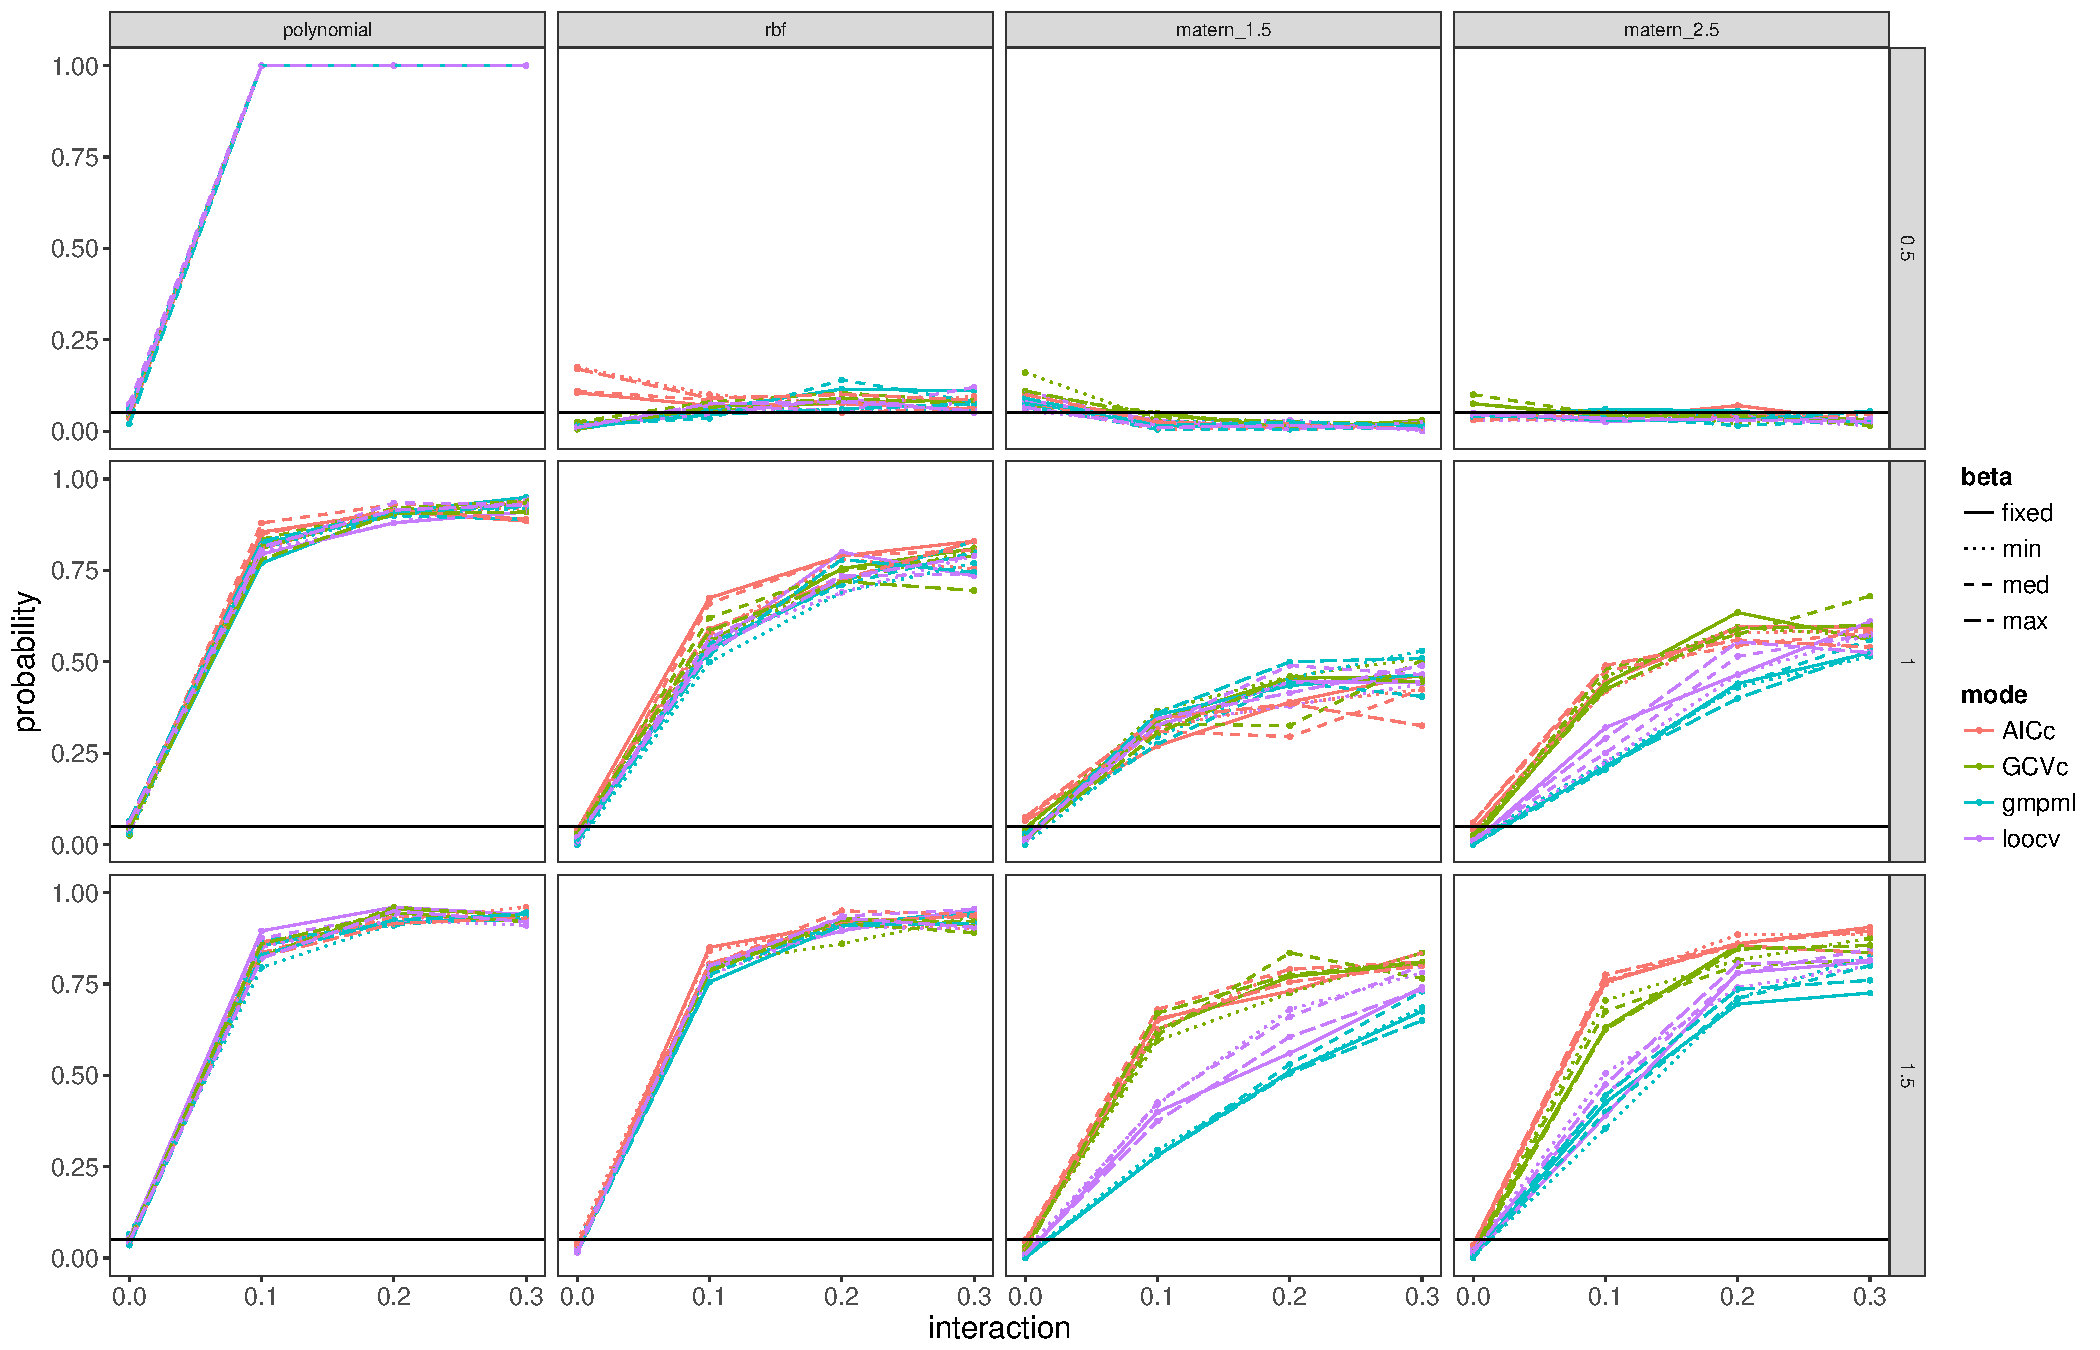
\includegraphics[width=0.9\columnwidth]{exp_A1} 
\caption{Asym, True kernel only}
\label{fig:res}
\end{center}
\end{figure}

\begin{figure}
\begin{center}
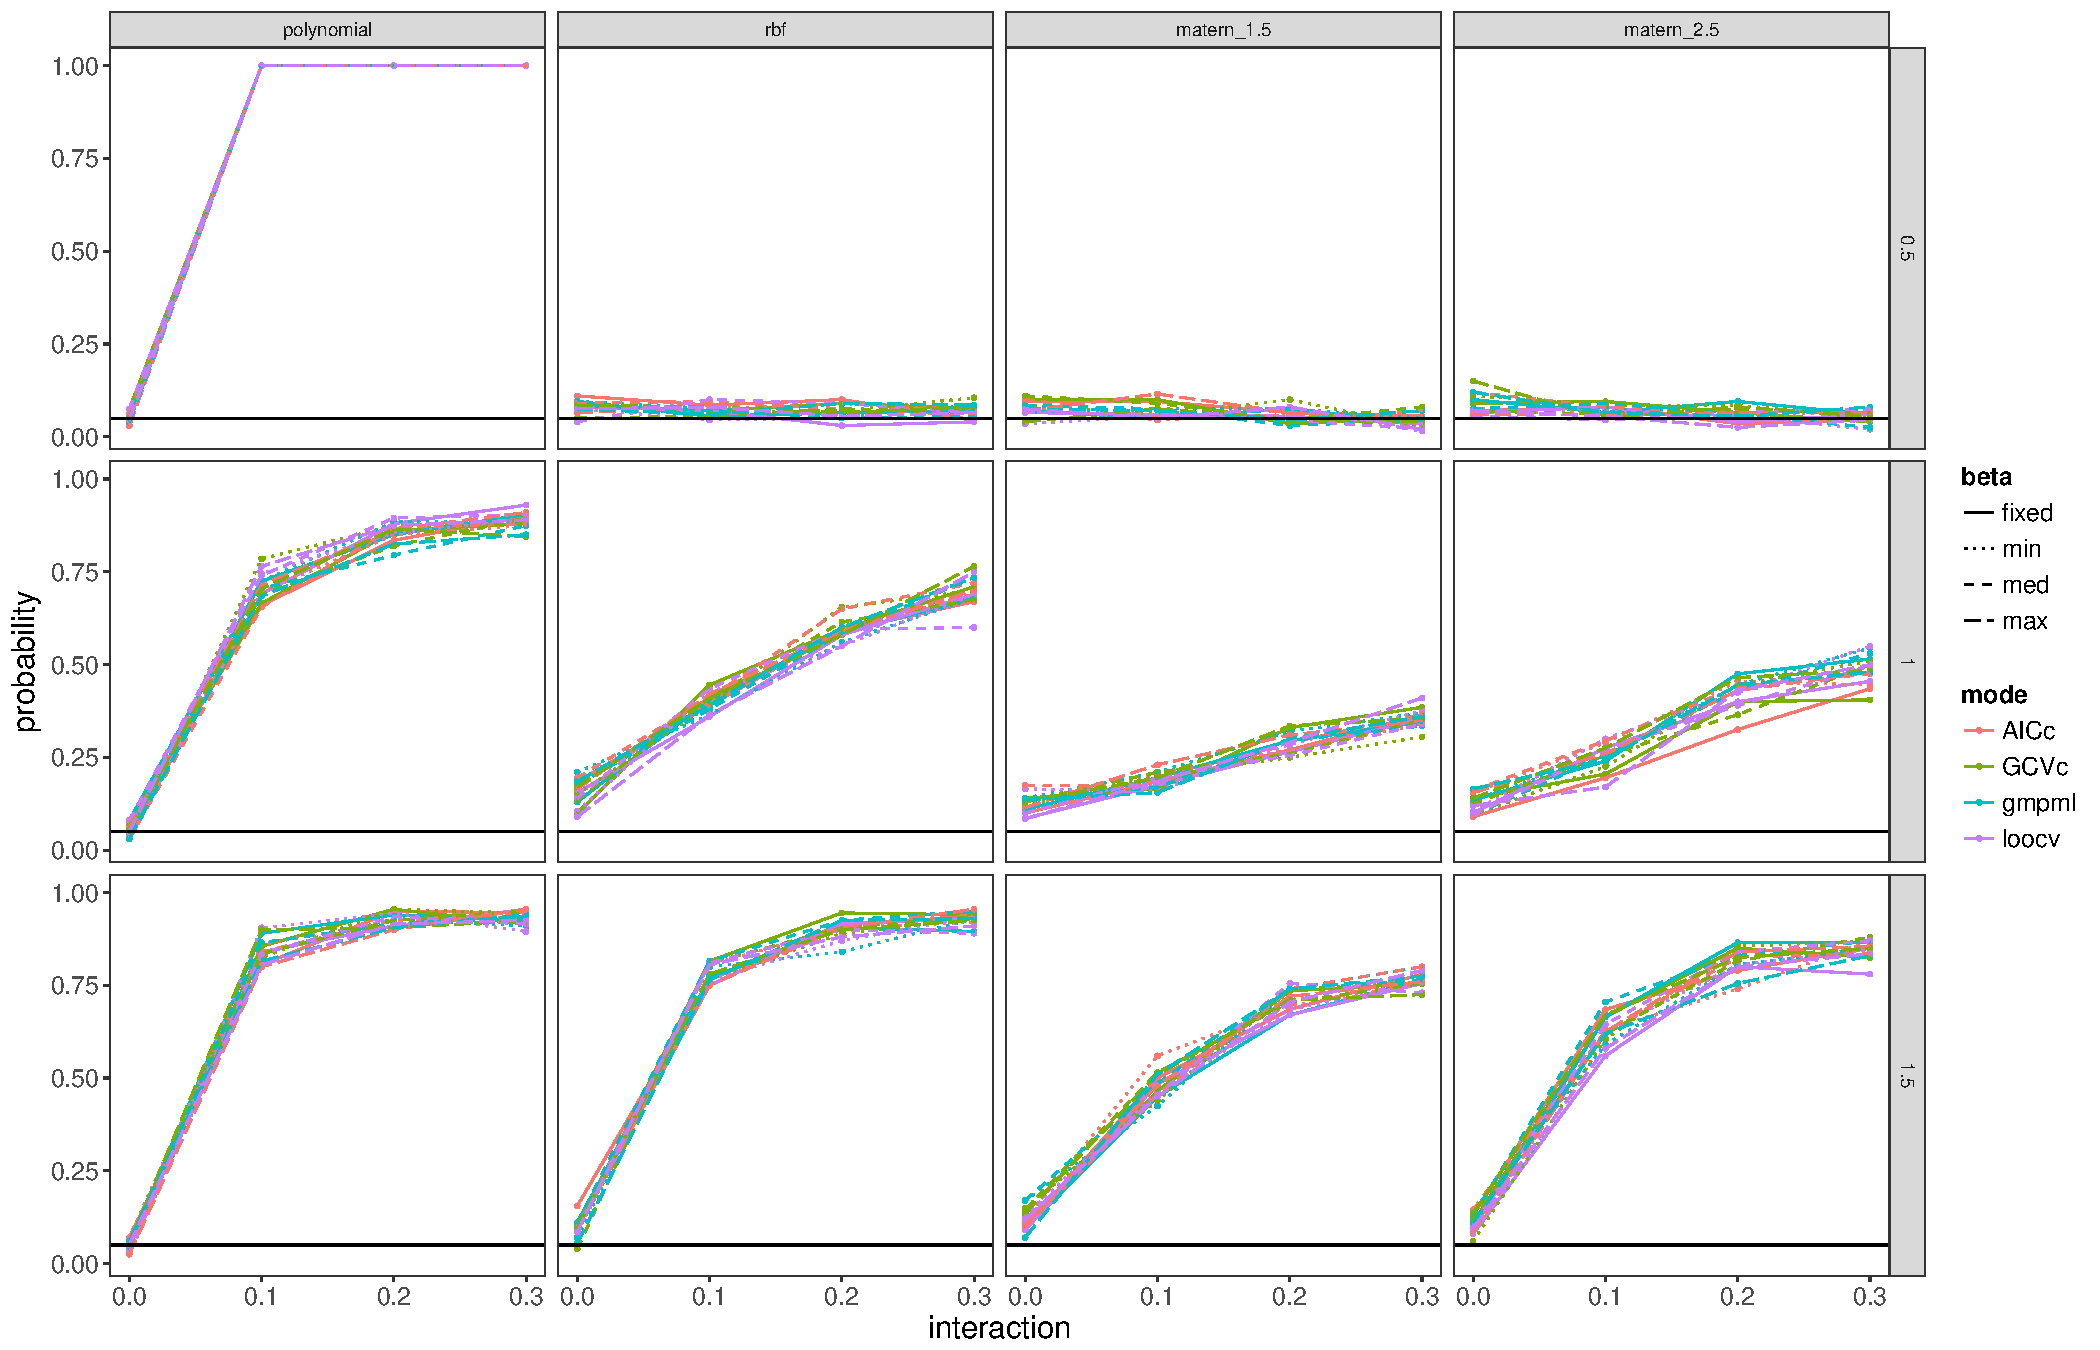
\includegraphics[width=0.9\columnwidth]{exp_A2} 
\caption{Asym, 3 Polynomial kernels}
\label{fig:res}
\end{center}
\end{figure}

\begin{figure}
\begin{center}
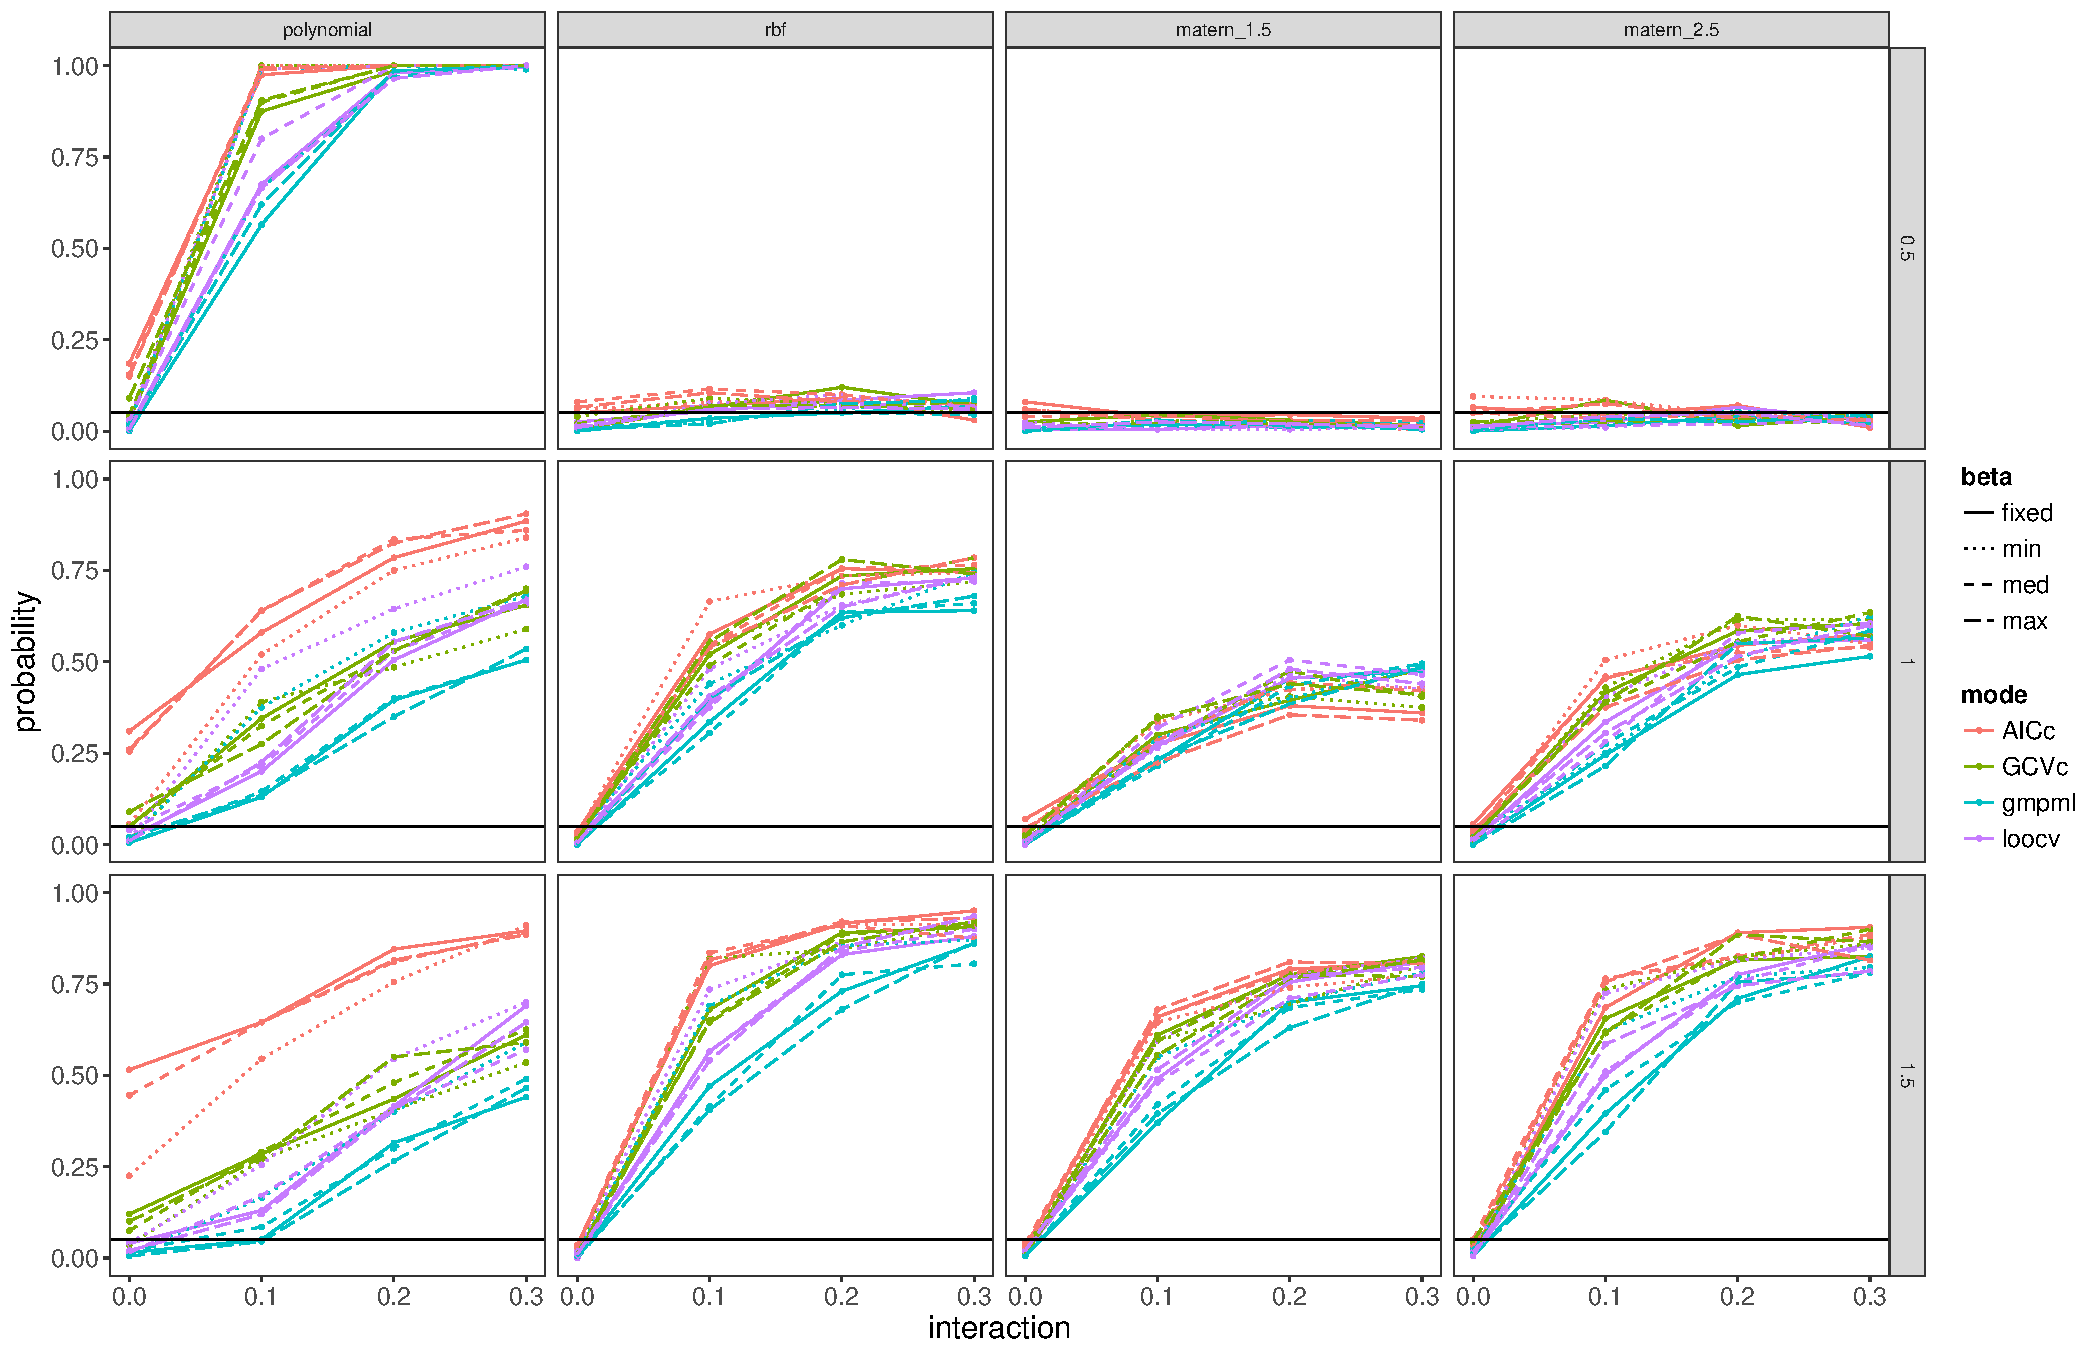
\includegraphics[width=0.9\columnwidth]{exp_A3} 
\caption{Asym, 3 RBF kernels}
\label{fig:res}
\end{center}
\end{figure}

\begin{figure}
\begin{center}
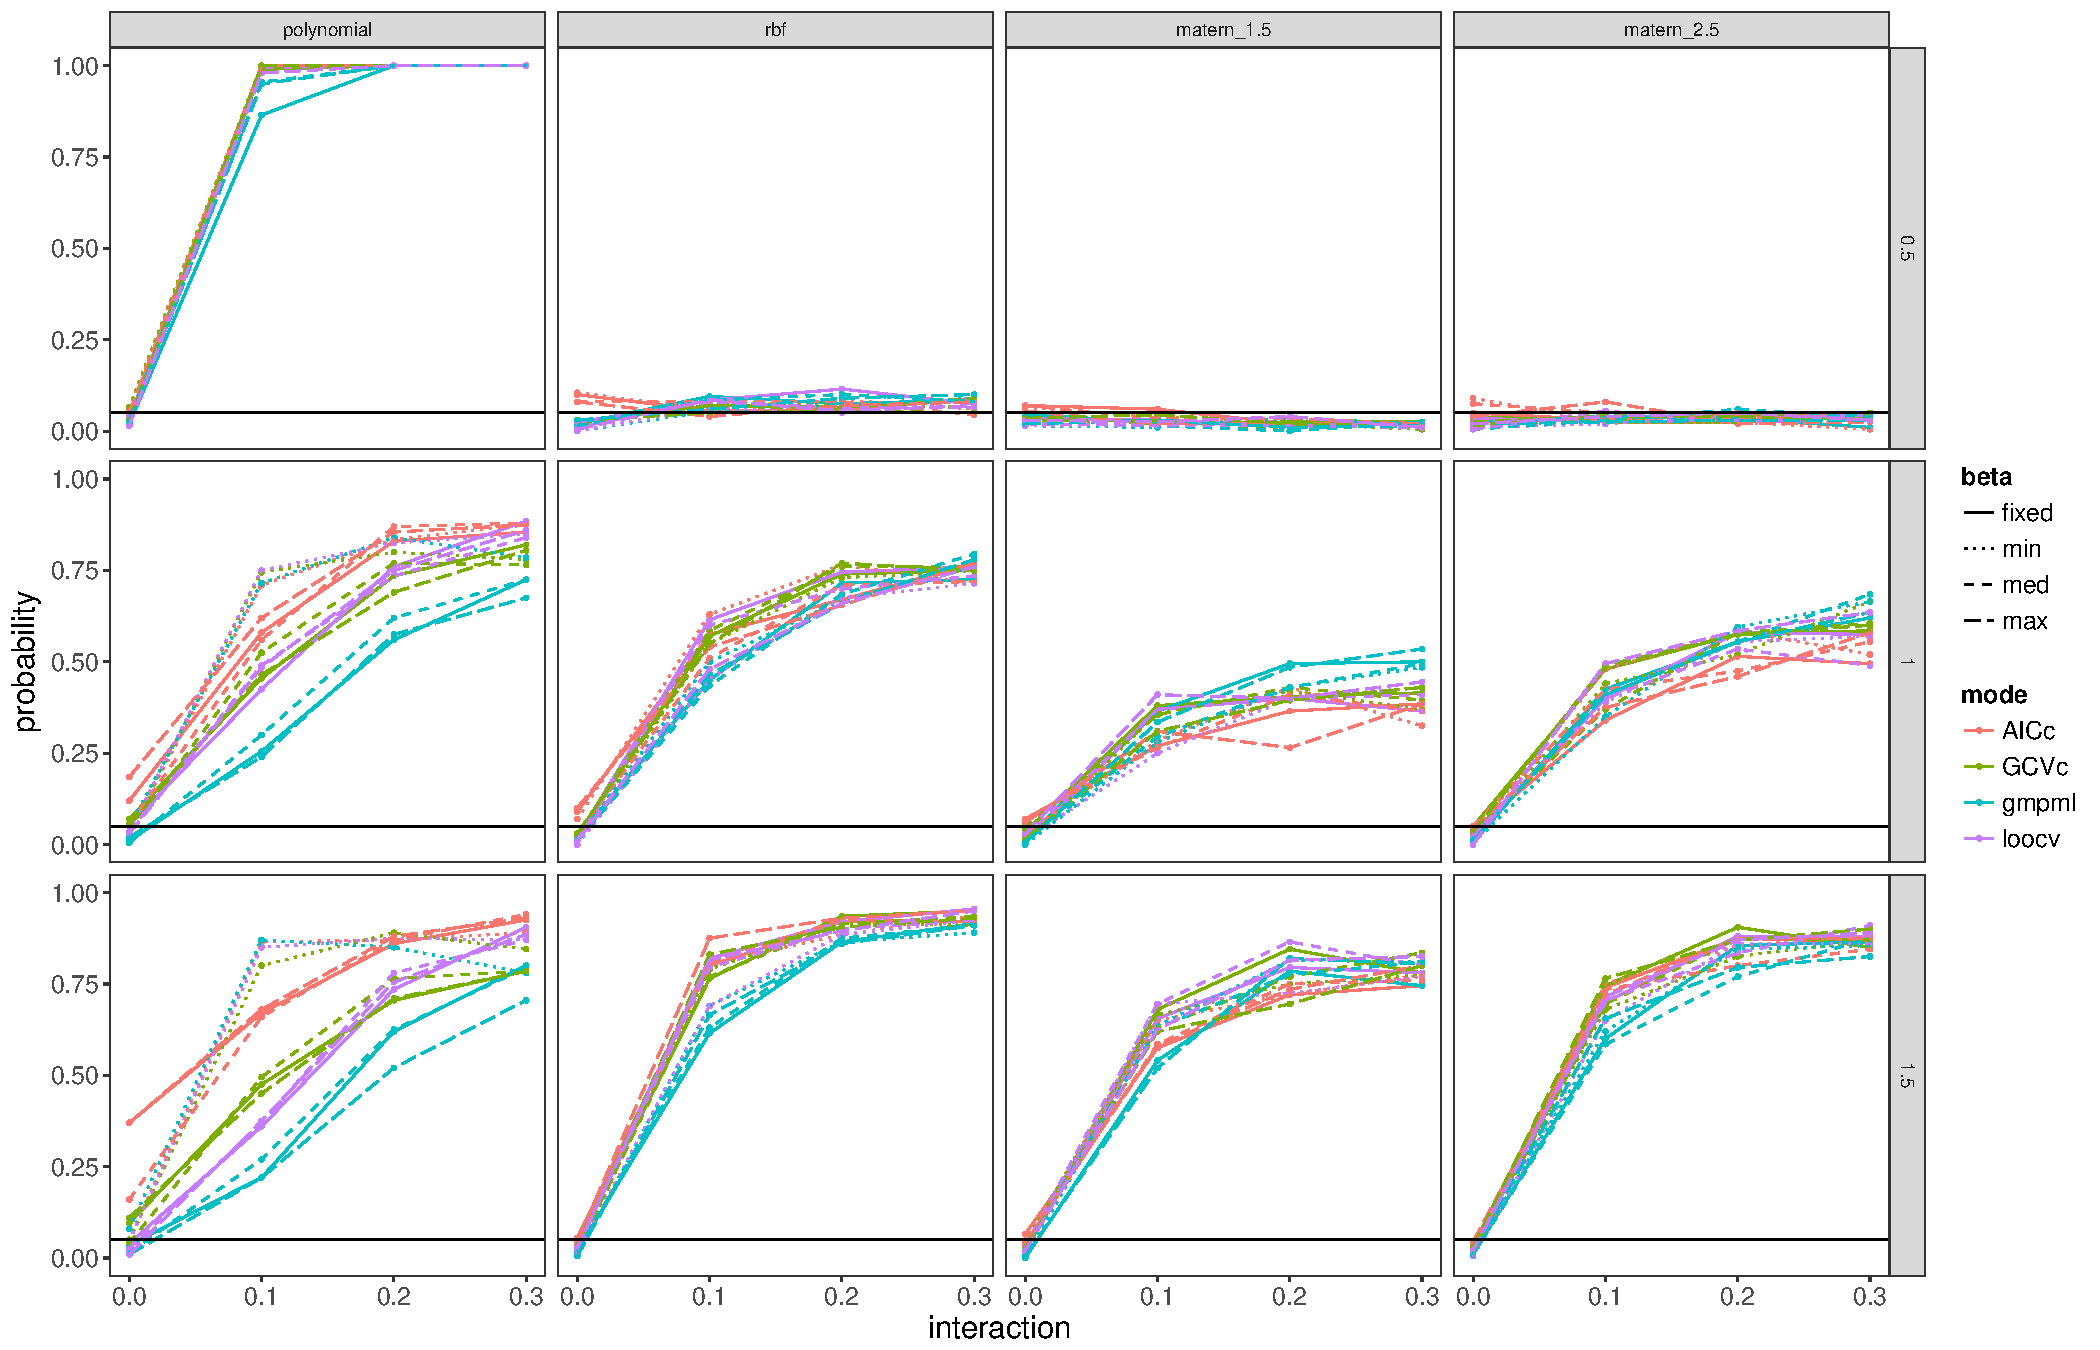
\includegraphics[width=0.9\columnwidth]{exp_A4} 
\caption{Asym, 3 Polynomial kernels and 3 RBF kernels}
\label{fig:res}
\end{center}
\end{figure}

\begin{figure}
\begin{center}
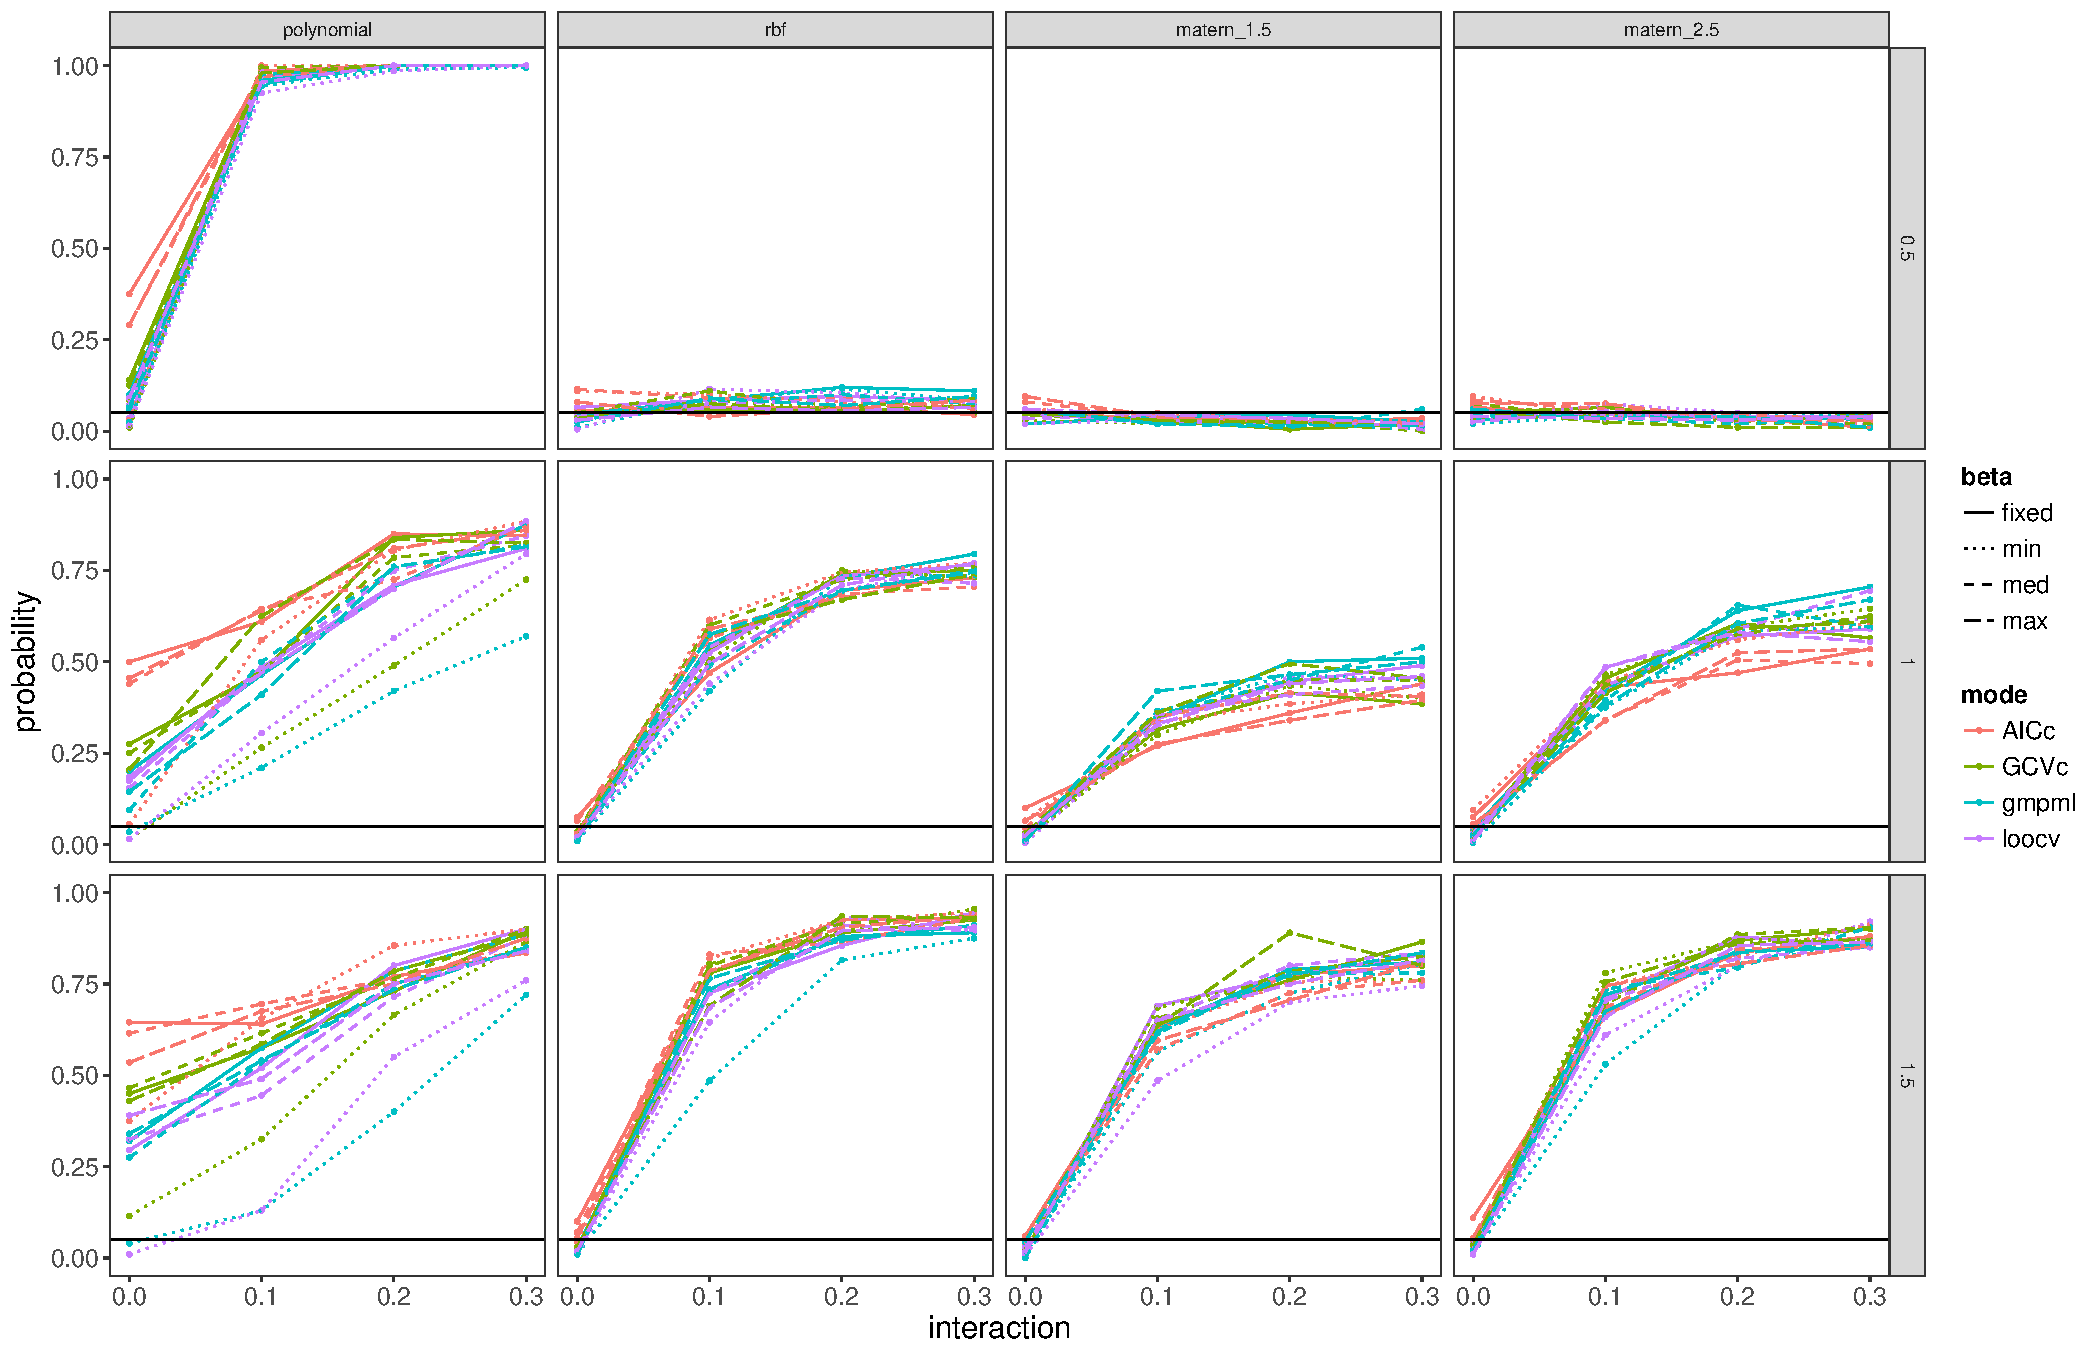
\includegraphics[width=0.9\columnwidth]{exp_A5} 
\caption{Asym, 3 Matern kernels and 3 RBF kernels}
\label{fig:res}
\end{center}
\end{figure}

\begin{figure}
\begin{center}
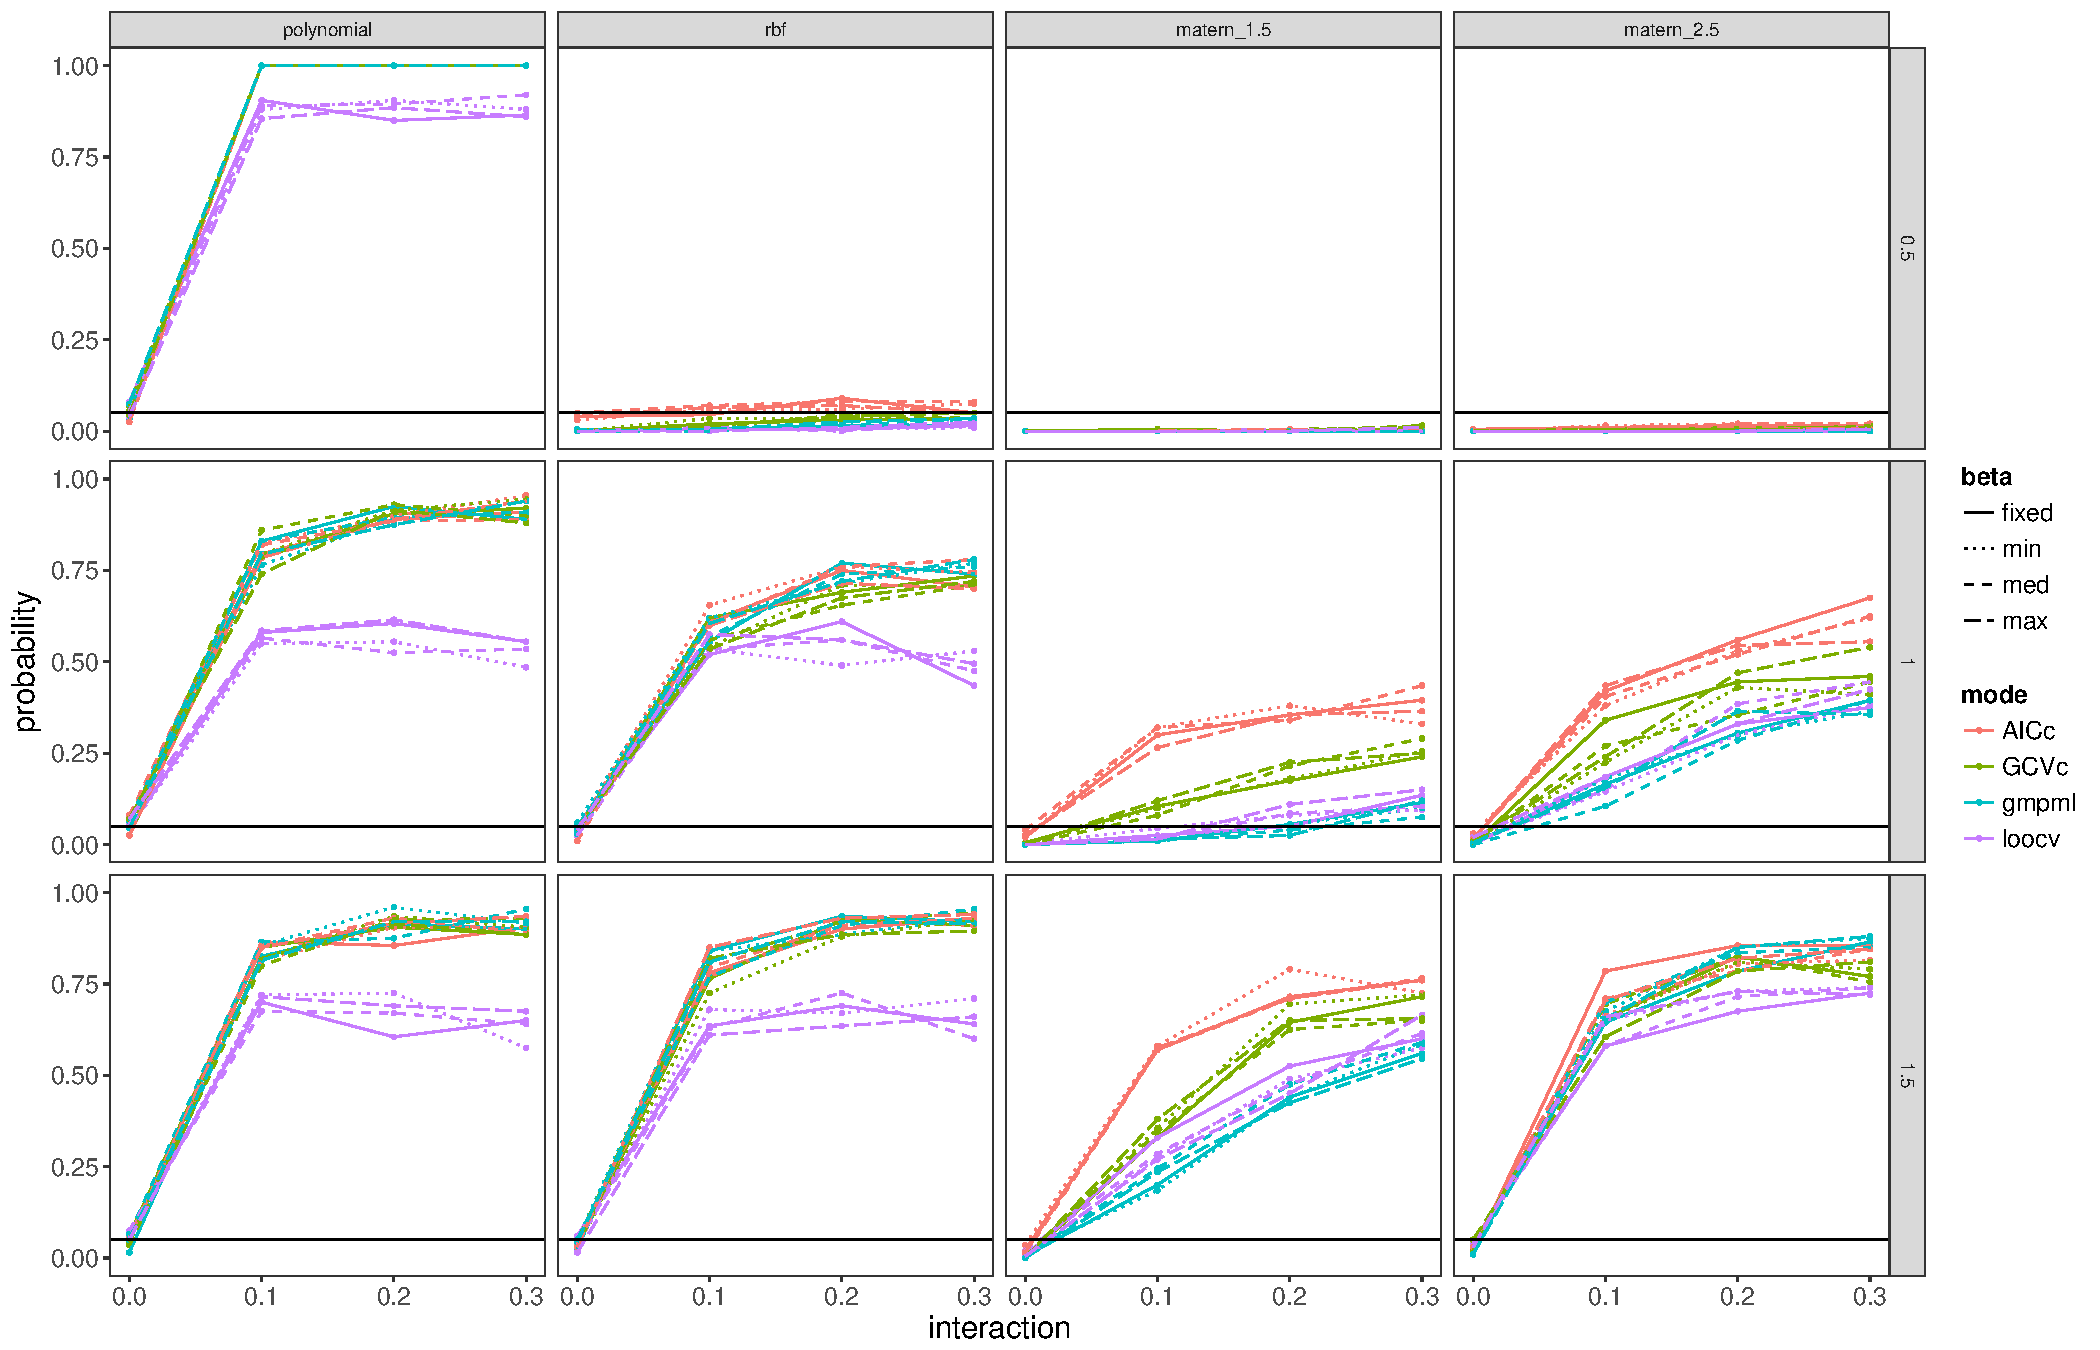
\includegraphics[width=0.9\columnwidth]{exp_B1} 
\caption{Boot, True kernel only}
\label{fig:res}
\end{center}
\end{figure}

\begin{figure}
\begin{center}
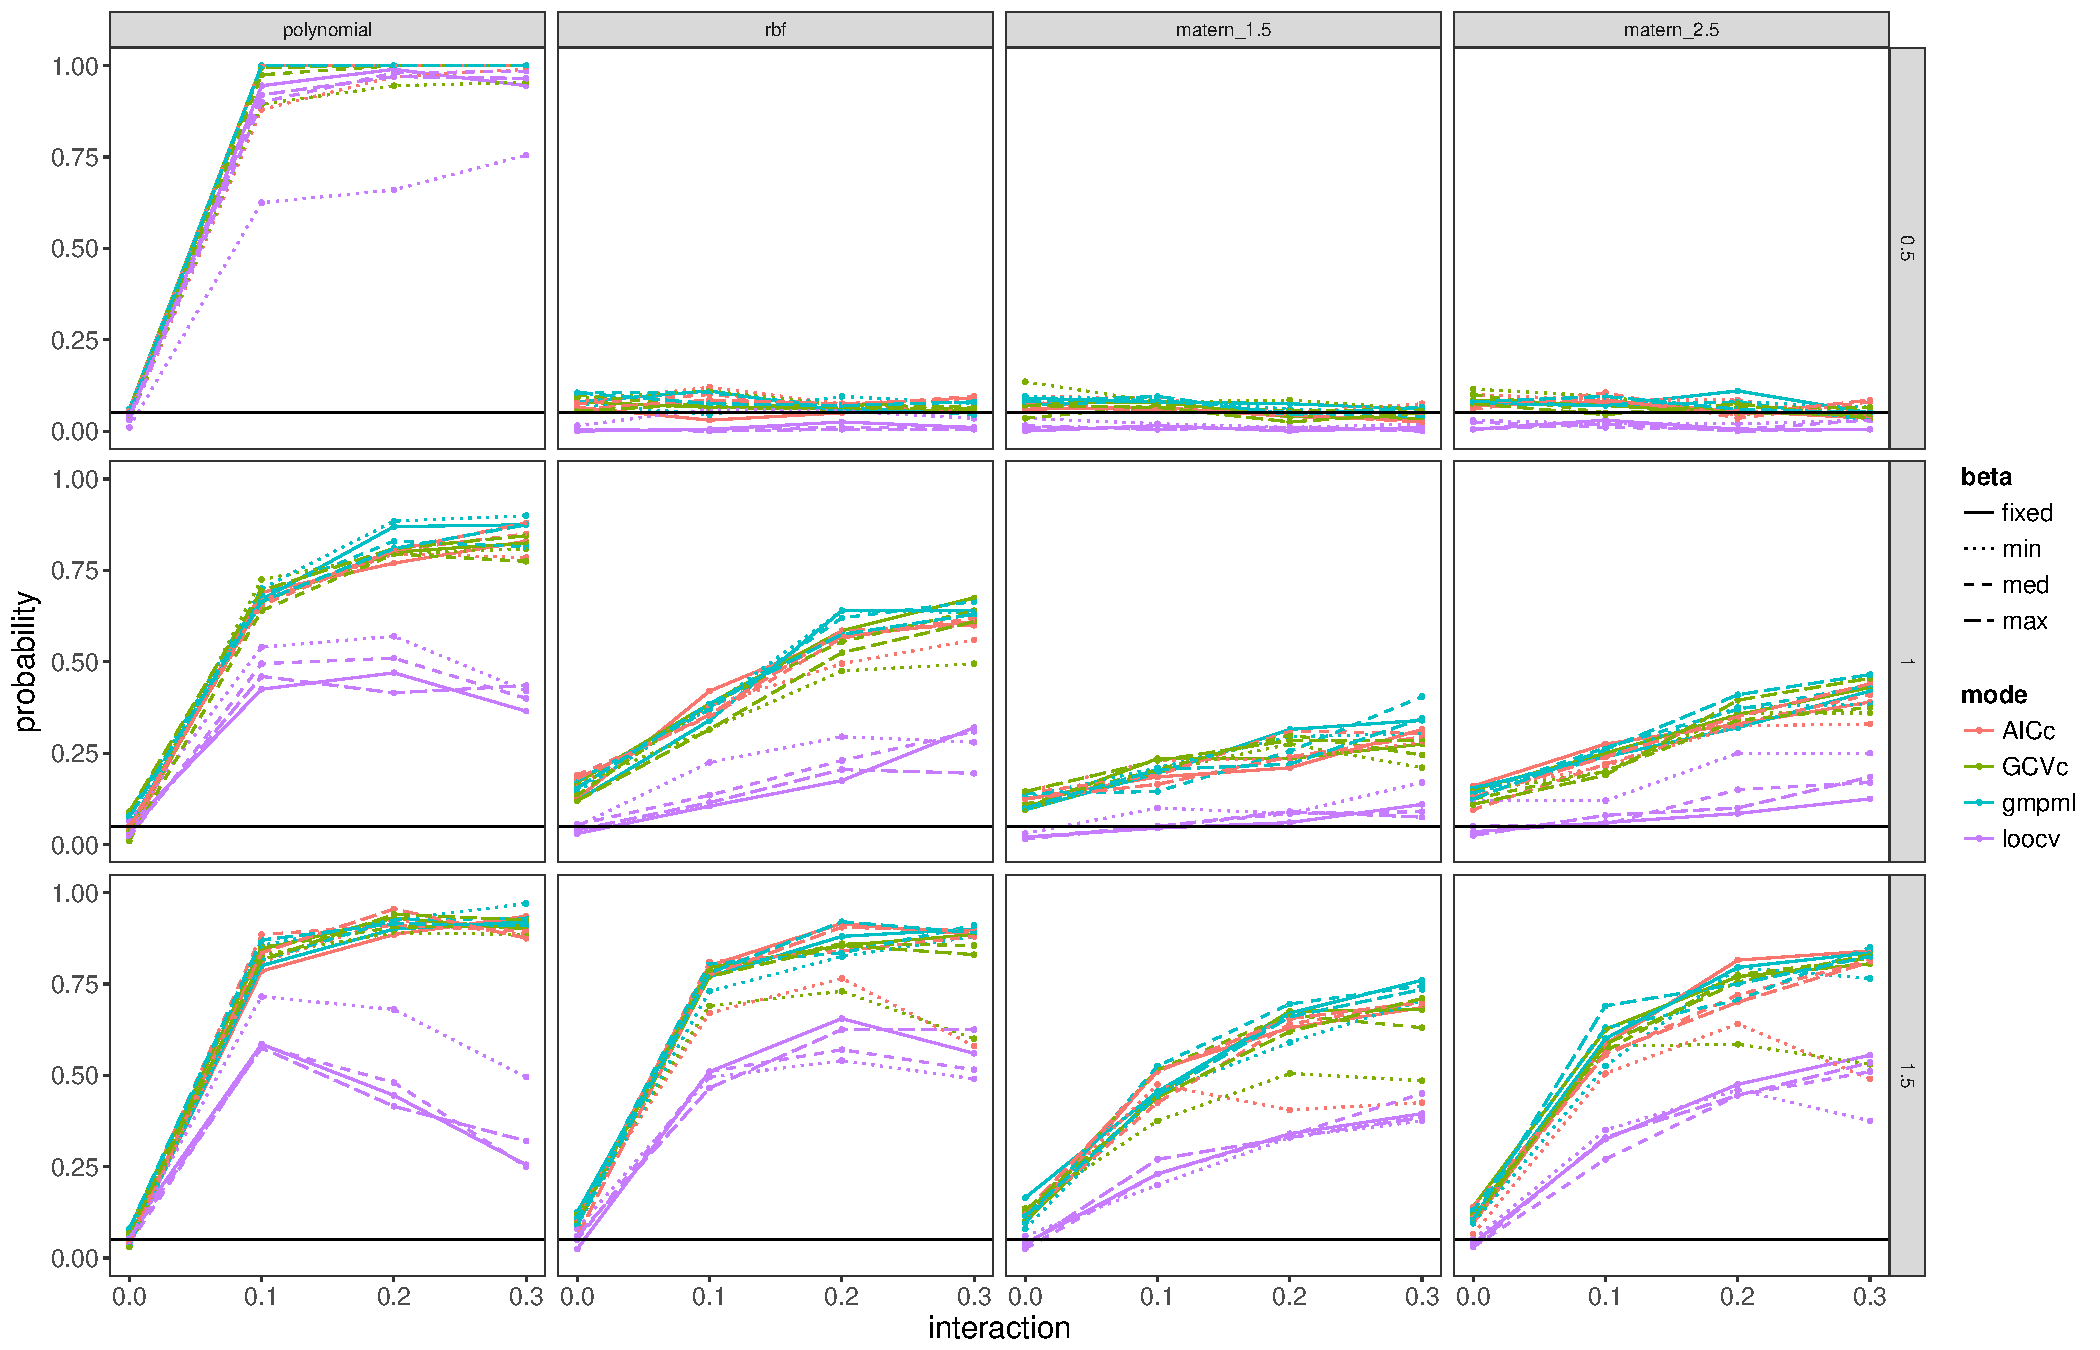
\includegraphics[width=0.9\columnwidth]{exp_B2} 
\caption{Boot, 3 Polynomial kernels}
\label{fig:res}
\end{center}
\end{figure}

\begin{figure}
\begin{center}
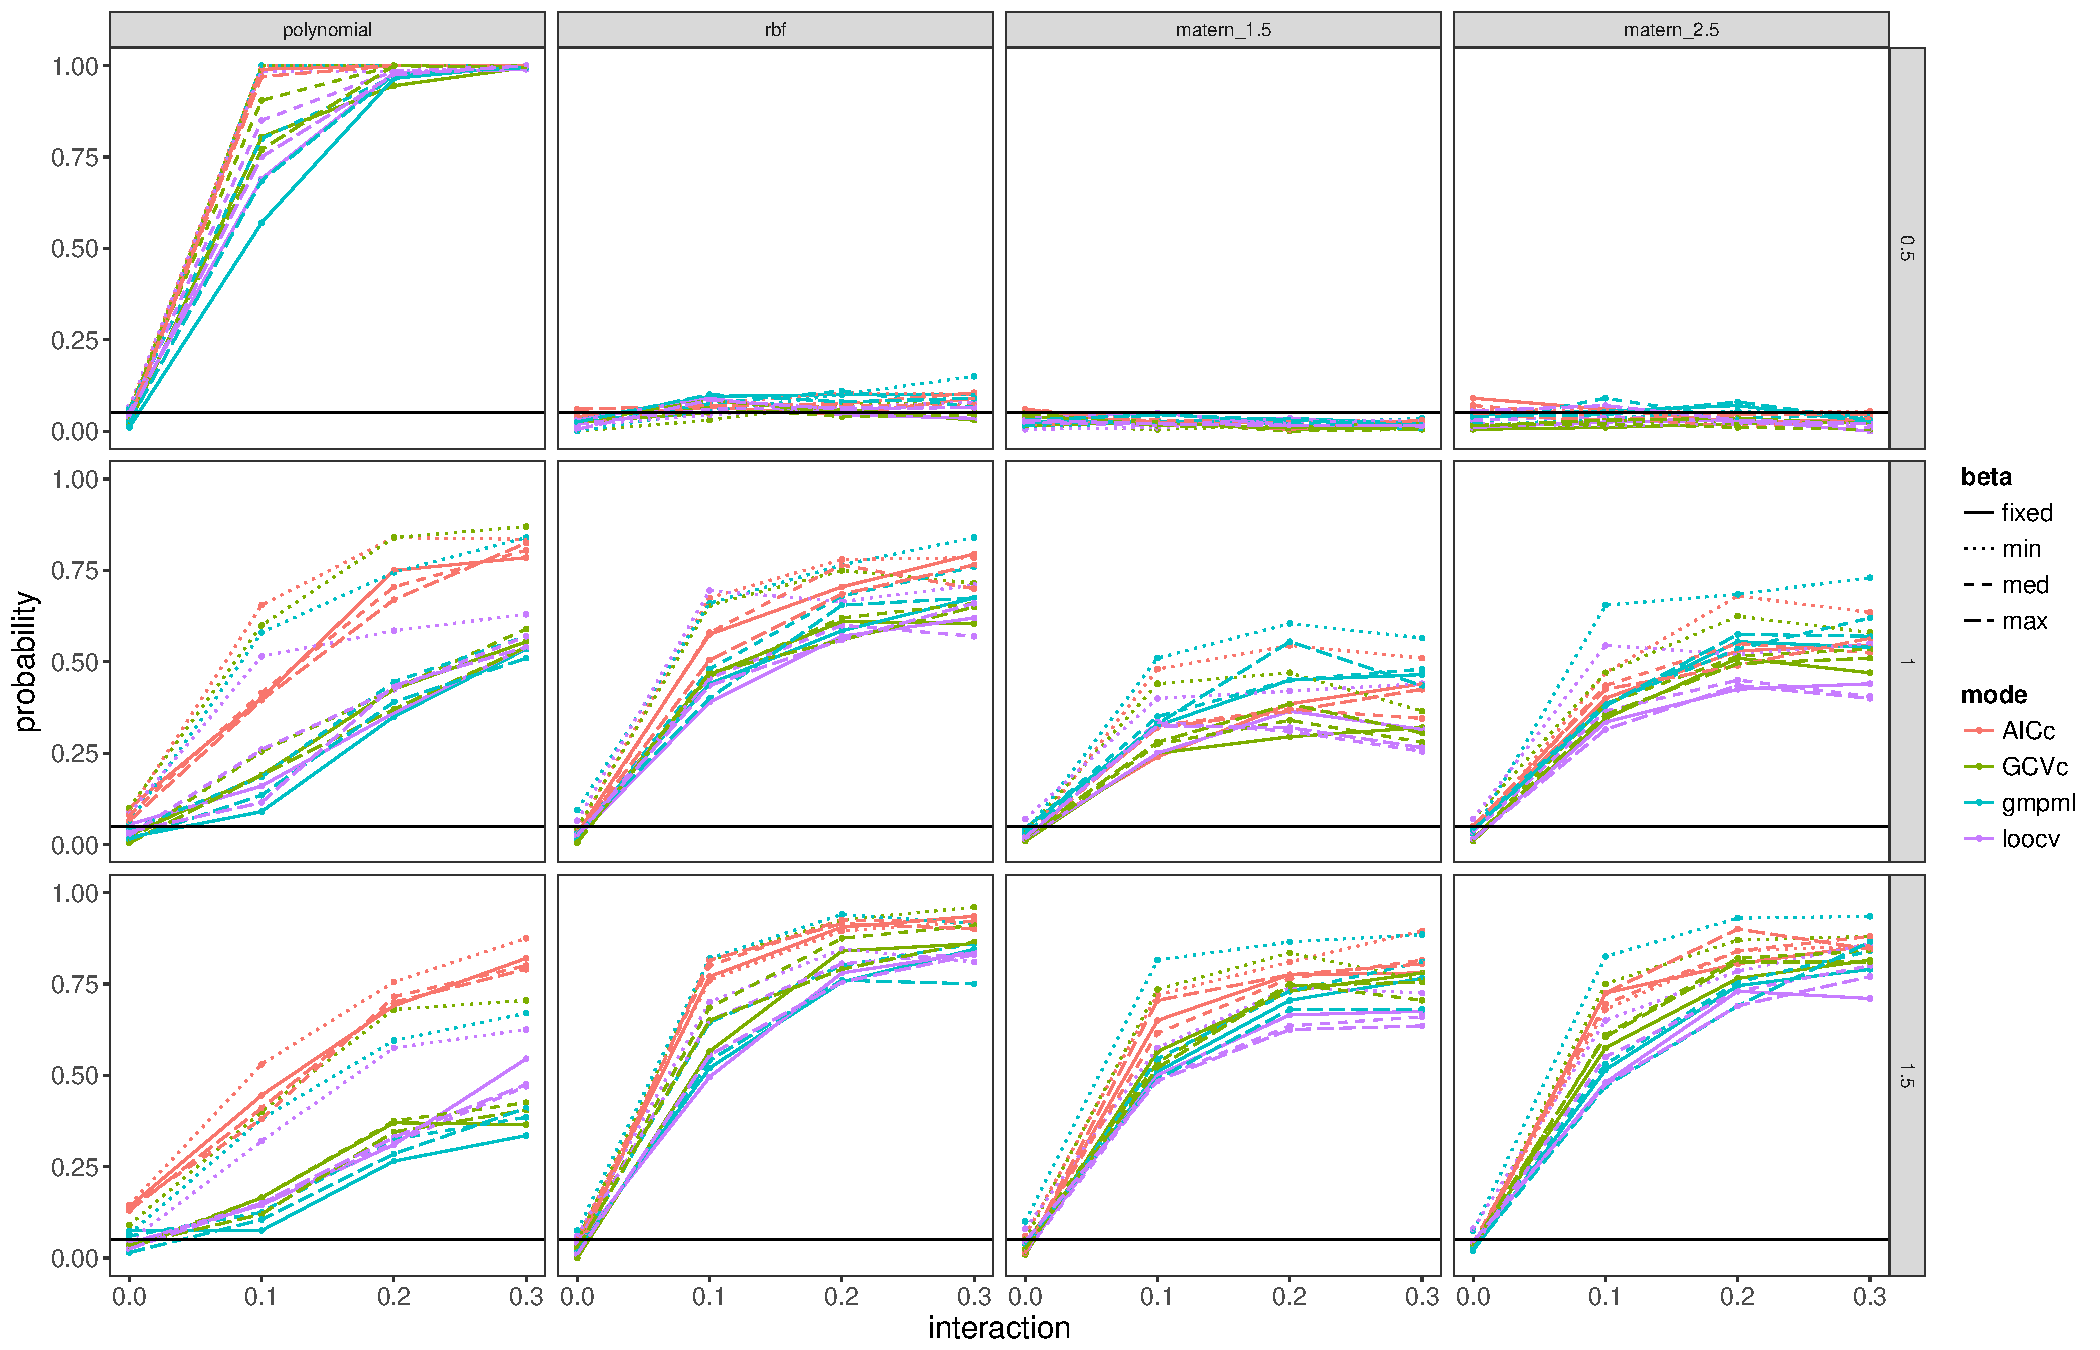
\includegraphics[width=0.9\columnwidth]{exp_B3} 
\caption{Boot, 3 RBF kernels}
\label{fig:res}
\end{center}
\end{figure}

\begin{figure}
\begin{center}
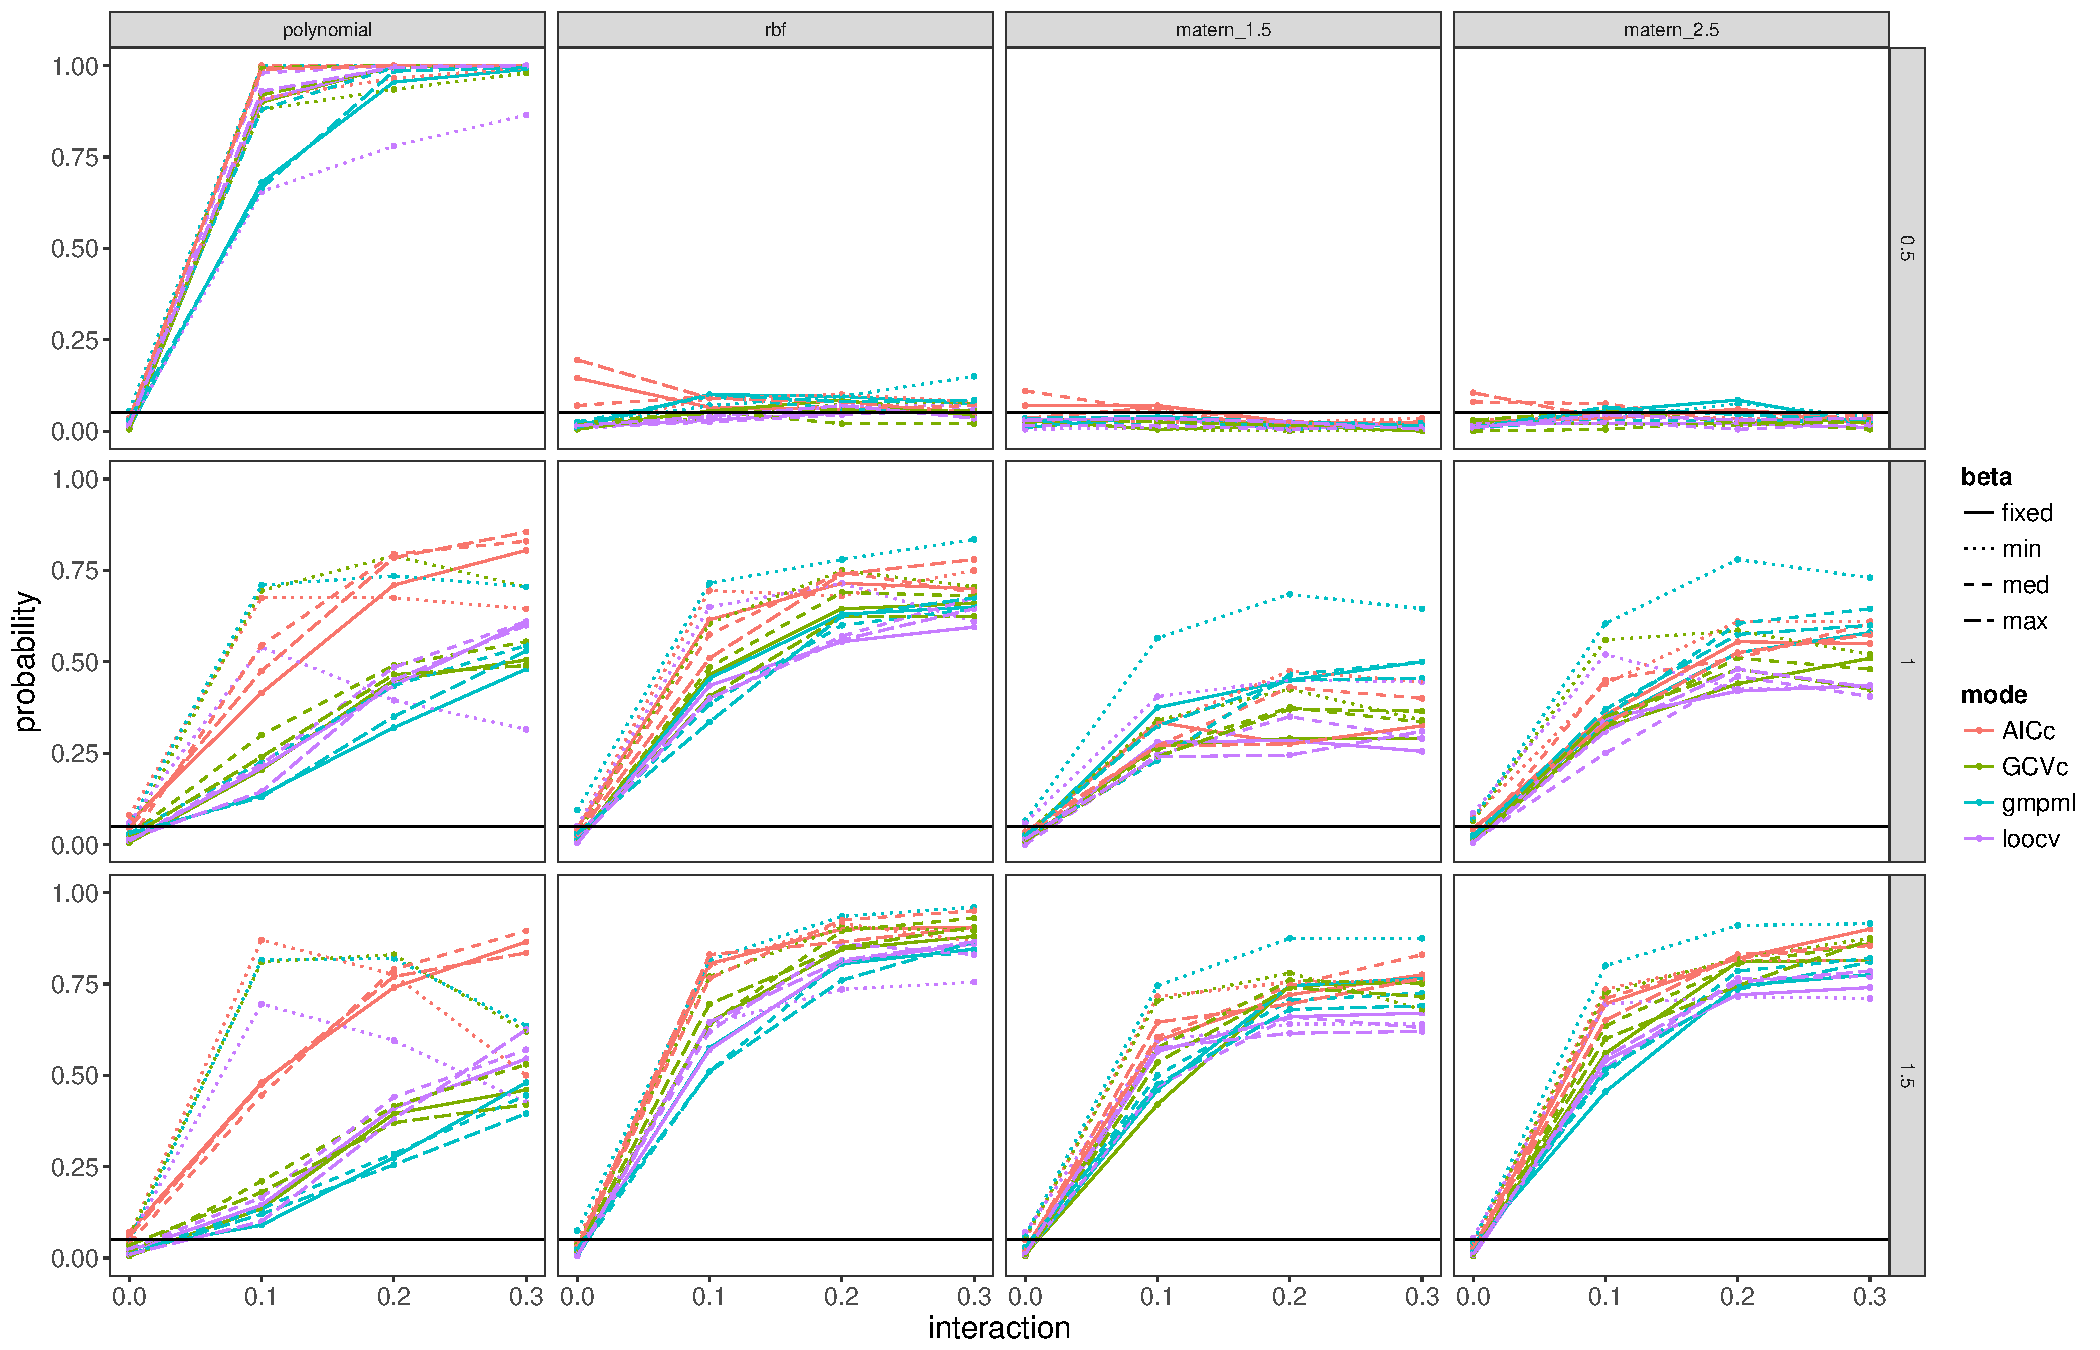
\includegraphics[width=0.9\columnwidth]{exp_B4} 
\caption{Boot, 3 Polynomial kernels and 3 RBF kernels}
\label{fig:res}
\end{center}
\end{figure}

\begin{figure}
\begin{center}
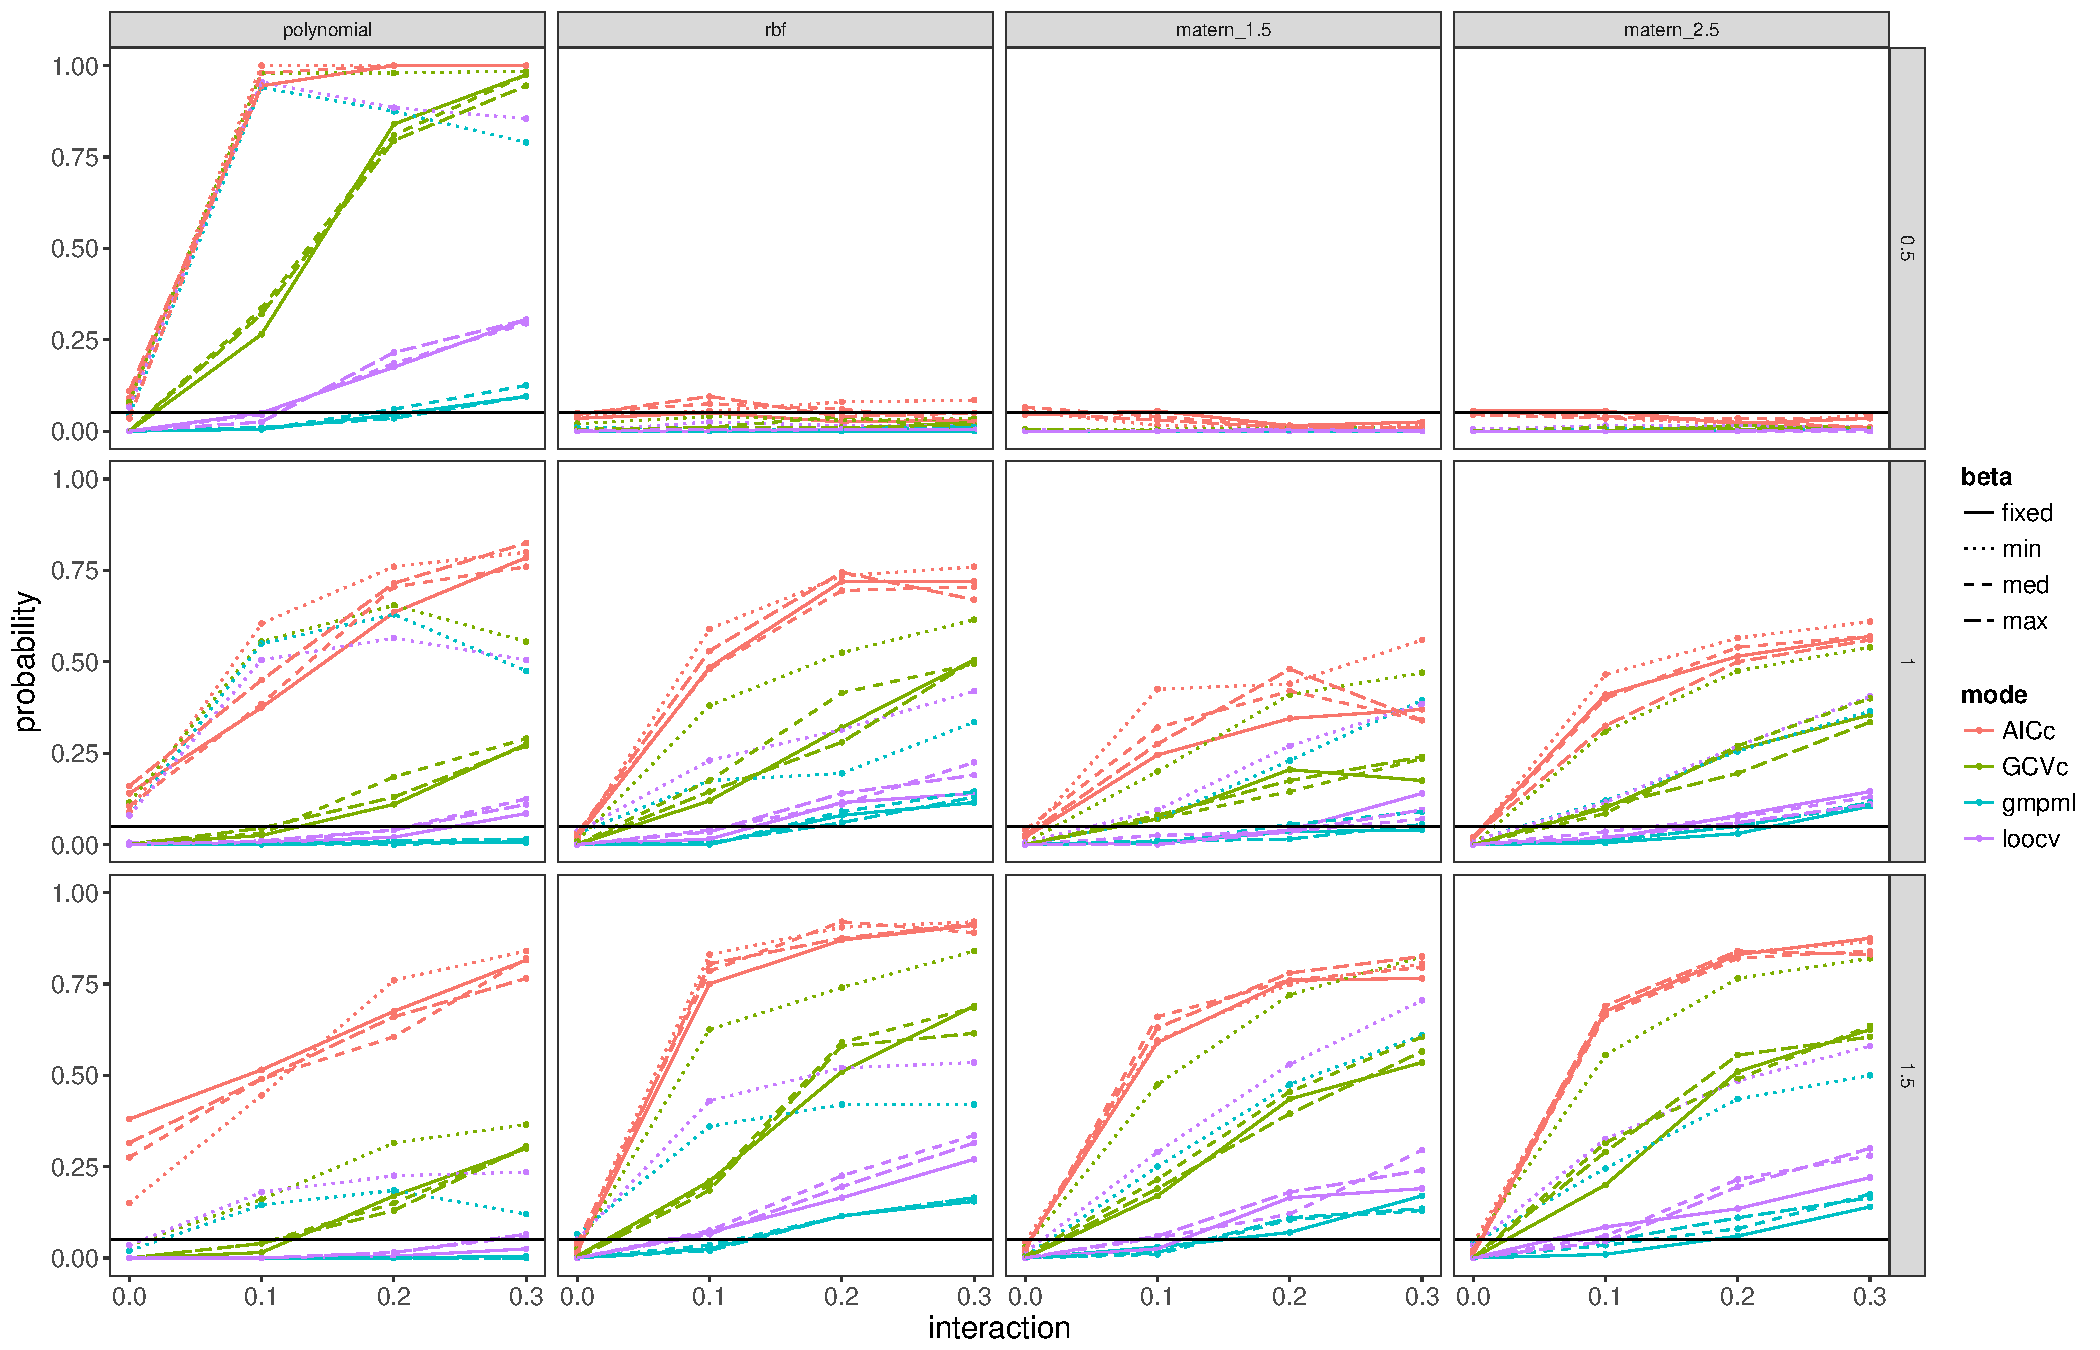
\includegraphics[width=0.9\columnwidth]{exp_B5} 
\caption{Boot, 3 Matern kernels and 3 RBF kernels}
\label{fig:res}
\end{center}
\end{figure}


\clearpage
\bibliography{reference2}


%----------------------------------------------------------------------------------------
\end{document}
